\documentclass{article}
\usepackage{setspace}
\usepackage{natbib}
\usepackage{amsmath}
\usepackage{float}
\usepackage{longtable}
\usepackage{booktabs}
\usepackage{lscape}
\usepackage{graphicx}
\usepackage{silence}
\usepackage{forest}
\usepackage{hyperref}
\usepackage{xr}
\usepackage{placeins}
\usepackage{textcomp} % Needed on Windows in Office
\usepackage{adjustbox}
\usepackage{xcolor}
\usepackage[letterpaper, margin=1in]{geometry}

\usepackage[toc,page]{appendix}


\let\Oldsubsection\subsection
% \renewcommand{\subsection}{\FloatBarrier\Oldsubsection}
\newcommand{\comment}[1]{}

\author{Ann Atwater\footnote{Department of Economics, University of Florida.}}
\title{Distributional Effects of Mergers: Evidence from the Attempted JetBlue-Spirit Merger\footnote{This is a preliminary draft. All errors belong to the author. The author would like to thank the participants of the University of Florida Applied Microeconomics working group and of the Southern Economics Association 2024 conference for helpful feedback. Furthermore, the author would like to thank Brad Shrago for alerting her to the reliance on usage fees by ultra-low-cost carriers. }}

\graphicspath{{05.Figures/}}

\begin{document}
	\maketitle
	
	\begin{abstract}
In 2024, the attempted merger between JetBlue Airways and Spirit Airlines was blocked following a lawsuit brought by the Department of Justice. I estimate the counterfactual pricing effects that would have resulted from this merger. I estimate that the average market price would have slightly increased following the merger. However, at least 35 air travel markets would have had the minimum market fare increase by over \$60 following the merger under even the assumptions most favorable to the merger's approval. Finally, I estimate that the merger would have increased consumer surplus had it been allowed to be completed, by at least \$350 million dollars. My results are as such mixed on the economic rationale for blocking the merger. Had the merger been completed, I estimate that it would have improved consumer welfare while at the same time forcing some consumers to exit air travel markets. These findings point towards complications in implementing the consumer welfare standard. \bigskip 

    \noindent JEL Classification: L4, L41 \newline
	\noindent Keywords: mergers; antitrust; airlines
		
	\end{abstract}
	
	\pagebreak
	
	\doublespacing
	
	\section{Introduction}
	\label{sec:Introduction} 
    Horizontal mergers between firms in the same industry can create a more efficient firm through the realization of economies of scale, the shifting of assets to more productive uses, and the sharing of productive technology \citep{williamson_economies_1968, farrell_horizontal_1990, kaplow_improving_2025}. Simultaneously, horizontal mergers result in a reduction in competition as the merging firms effectively become fully coordinate their production decisions post-merger \citep{stigler_theory_1964}. As such, horizontal mergers ambiguously change both consumer and societal welfare. Incorporating this insight into public policy, virtually all anti-trust regulators operate under the  ``consumer welfare" standard for approving mergers: for regulators to approve mergers that represent large reductions in competition, the merging firms must demonstrate efficiencies sufficient to offset the impulse to raise prices and harm consumers \citep{whinston_chapter_2007}. % This standard has come under attack by the ``Neo-Brandesian" movement of lawyers within the last decade, who believe that effective antitrust policy requires the movement to more restrictive merger approval regimes focused on combating the formation of large firms regardless of potential harm to consumers. During the Biden Administration, the head of the Federal Trade Commission and the head of the Department of Justice's antitrust division would be members of this intellectual movement. 

    Certain industries have firms offering lower quality goods at lower prices than the competition, such as discount grocers. While these firms are not necessarily the largest, they allow cost pressured consumers who would otherwise be unable to afford certain goods to consume them. Within the airline industry, low-cost carriers and ultra-low-cost carriers fit this model. In 2022, JetBlue Airways, a low-cost carrier, attempted to acquire Spirit Airlines, the largest ultra-low-cost carrier in the United States. Notably, JetBlue indicated its desire to retire Spirit's business model targeting extremely price-conscious travelers.   This motivated the Department of Justice to sue to block the merger. In his decision, Judge William G. Young chose to block the merger due to the belief that these particular consumers would face harm from the merger and as such the merger would violate the Clayton Act \citep{william_g_young_findings_2024}. My paper estimates the counterfactual pricing effects of the JetBlue-Spirit merger to examine the effects of the merger in more detail. 
    
    % Broadly speaking - need to introduce key point - market segmentation may lead to mergers which can increase overall consumer surplus while still negatively impacting constrained consumers. 

    As the JetBlue-Spirit merger was never completed, I  use structural modeling to estimate the pricing effects that would have been realized had the merger been completed. I first model supply and demand for air travel products within the continental United States. I estimate demand using a random coefficient nested logit model and supply as being using Bertrand Competition. This allows me to recover product level marginal costs which I then use simulate the merger effects across three separate specifications which can be thought of as a ``best case" for the merger, an ``average case" for the merger, and a ``worst case" for the merger. To check the robustness of my results to the impact of the concurrent Northeast Alliance between JetBlue and American Airlines and post-pandemic changes to the industry, I conduct these analyses separately on two samples: one consisting of the three years prior to the COVID-19 pandemic and one consisting of the two years following the resumption of mass air travel in 2021 following widespread vaccine availability. 

    I estimate that the average markets with both firms would have seen substantial declines in average prices within the best case simulation and only minor increases of between 4-5\% under the other two simulations. However, I estimate that under all three scenarios, at least thirty-five markets in each period would have experienced increases in the minimum market fare of at least \$60. Under the worst-case scenario, this number increases to over two hundred markets within each sample. This is notably consistent with the judicial ruling despite my sample excluding markets touching on Puerto Rico, which were identified as being particularly vulnerable to price increases had the merger been approved. It is worth noting that the base fares offered by Spirit Airlines are typically among the cheapest available. In line with this, I examine the change in the minimum fare available within JetBlue-Spirit markets within my simulations.

    I then expand on this analysis by analyzing changes in consumer surplus on my primary data set and an additional one intended to adjust the Spirit fares to be closer to the true fares paid after ancillary fees are included. In both, I find that the merger was liable to have decreased (increased) overall consumer surplus had it been consummated in the period before (after) the pandemic. In conjunction with my findings on the minimum market fair effects of the merger, this points to the merger having positive effects for consumers on the interior margin while potentially having negative effects for consumers on the exterior margin. 

    % Contribution 2 - Different Merger Focus

    The existing literature is divided on the net price effects of the wave of mergers that have occurred within the airline industry since the turn of the century. This division is due to differences in both merger characteristics and study methodology. To understand the impact of different methodologies on the estimated pro- or anti-competitive price effects, consider \citet{luo_price_2014} and \citet{carlton_are_2019}. These papers estimate pro-competitive effects of the United-Continental merger by using a differences-in-differences inference design which relies on the determination of pre- and post-periods. By contrast, \citet{fan_when_2020} finds evidence for price increases following this merger through the adoption of a model that allows for the realization of dynamic price effects following mergers. The dynamic price effects model provides evidence consistent with prices rising following key merger milestones other than completions. Research, such as \citet{bet_retrospective_2021, ciliberto_market_2021}, using structural modeling to recover firm marginal costs and markups to analyze the effects of these mergers has found similarly mixed evidence for the effects of mergers. \citet{bet_retrospective_2021} found evidence for increases in markups resulting from the United-Continental, Southwest-AirTran, and American-US Airways mergers but not the Delta-Northwest merger due to limited efficiency gains across these mergers. \citet{ciliberto_market_2021} estimated the effects of the American-US Airways merger using a structural model allowing for firms to reposition their product offerings following the completion of the merger. Through this model, they estimate price increases of around 5\% for duopoly markets consolidated by the merger. This is similar to my estimates for the average JetBlue-Spirit market under the ``average case" and ``worst case" simulations despite these firms' smaller market shares. However, I build further on this by estimating how the entire distribution of fares would change, and find that minimum market fares would have faced higher increases had the merger been approved. % My model is structural

    % Contribution 3 - Description

    Finally, through the use of more recent data, I examine the evolution of the airline industry through the period following the COVID-19 pandemic. I find that despite the documented decline in business travel caused by the pandemic, demand only became slightly more elastic post-pandemic, consistent with research estimating less price sensitivity among leisure travelers post-pandemic \citep{ewen_zoom_2023}. Furthermore, I document changes in the role that low-cost carriers and ultra-low-cost carriers play within the industry. Historically, low-cost carriers and ultra-low-cost carriers have only rarely competed in the same markets \citep{ciliberto_market_2021}. Despite this, within my sample, there exists a market with more than two low-cost carriers for every two markets with only a single low-cost carrier within it. This is consistent with the large growth of these carriers over the course of the previous decade.
    
    With these findings outlined, I will briefly discuss the structure of the remainder of the paper. Section \ref{sec:Setting} details the economically relevant features of consumer airlines and the proposed JetBlue-Spirit merger. I detail the data used within the analyses of this paper and present summary statistics within Section \ref{sec:Data}. I analyze the JetBlue-Spirit merger within Section \ref{sec:Analysis}.  I briefly conclude my paper in Section \ref{sec:Conclusion} with a brief discussion of the findings of this paper and examination of their implications for antitrust policy. 

  
	
	\section{Empirical Setting}
	\label{sec:Setting}
	
	\subsection{United States Airline Industry}
	\label{sec:Setting_Aviation}
	Three major types of airlines operate within the United States: legacy carriers, low-cost carriers, and ultra-low-cost carriers. This paper studies a proposed merger between JetBlue (a low-cost carrier) and Spirit (an ultra-low-cost carrier). Within this section, I detail the differences in firm structure for each of the three types of firm before describing JetBlue and Spirit in more detail.
    
	Legacy carriers operated interstate air service prior to fare deregulation in 1978. Delta, American, and United are the only legacy carriers still operating after a series of mergers occurred over the last few decades. These carriers operate hub-and-spoke route networks which require customers to connect through centralized hub airports to reach smaller destinations. These firms use more varied fleets than the other carrier types so that they can serve a wider variety of market types. While this practice allows for the servicing of smaller markets with lower excess capacity than if they flew uniform fleets, the additional variety in aircraft leads to additional crew training and maintenance expenditures.    
	
	Non-legacy airlines are divided into two groups: low-cost carriers and ultra-low-cost carriers. Low-cost carriers include Southwest and JetBlue, while the ultra-low-cost carriers are comprised of Spirit, Allegiant, and Frontier.\footnote{Alaska Airlines and Hawaiian Airlines are larger carriers with a regional focus. They operate a model closer to legacy carriers than that of low-cost carriers. Furthermore, there exist several smaller, more regional-focused low-cost carriers, such as Sun Country, that represent fringe supply within the industry. Later analyses within this paper treat products from these airlines as if they were offered by a single ``other" airline.} Low-cost carriers and ultra-low-cost carriers use route structures that are less centralized than those of legacy carriers (eschewing the use of hub airports) and more concentrated on serving the largest air travel markets. As such, more of these firms' customers fly on direct itineraries than customers of legacy carriers. This alternative route structure allows these carriers to avoid expenditures relating to the operation of hub airports and additional plane models. As such, fares for low-cost and ultra-low-cost carriers are typically lower than those for competing products offered by legacy carriers.

	Ultra-low-cost carriers are distinguished from low-cost carriers through the practice of ``unbundling," wherein base ticket prices are lower but amenities traditionally included within the price of a ticket are additional purchases. While Ryanair in Europe has operated under this model since the 1990s, a United States firm would not successfully adopt the strategy until Spirit introduced fees for checked baggage in 2010 \citep{bachwich_emergence_2017}. The total revenue derived from these fees is immense, and have come to represent about an even share of Spirit's revenue as the base ticket prices (Figure \ref{fig:Spirit_Revenue_Sources}). While complaints regarding the quality of these airlines are well documented in consumer surveys and the press \citep{vasel_spirit_2016, elliott_jetblue_2022}, these airlines have managed a degree of success by targeting highly budget-conscious travelers who do not wish to pay more expensive fares. By the later part of the 2010s, trips on ultra-low-cost carriers represented over a tenth of total air travel within the United States.  Despite this growth, the industry is still dominated by the ``big four" carriers - the three legacy carriers who along with Southwest comprise approximately three-quarters of the overall passenger trips within the United States. 

    Spirit rapidly grew within the post-recession domestic aviation landscape following its adoption of the ultra-low-cost carrier model and by the end of my sample period it served 8 million quarterly passengers (Figure \ref{fig:Quarterly_Pass_JB_SP}). To serve these passengers, Spirit grew its fleet from under 50 planes before adopting the ultra-low-cost model to nearly 200 planes by 2022 (Figure \ref{fig:Both_fleet}).\footnote{As depicted in the aforementioned figure, JetBlue's fleet stagnated following the pandemic due to it negotiating delayed fulfillment of orders placed before the pandemic \citep{bellamy_iii_jetblue_2020, sipinski_jetblue_2020}. JetBlue publicly stated that it viewed the proposed Spirit merger as a way to increase its fleet size despite the delayed orders.}  As part of this expansion in operations, Spirit increasingly competed against JetBlue (Figure \ref{fig:JBSpirit_Airports_2022}). This trend is especially notable as very few markets have historically had multiple low-cost carriers operating within them \citep{kwoka_fringe_2016, ciliberto_market_2021}. However, within my sample, I observe approximately one market with multiple low-cost or ultra-low-cost carriers for every three markets with a single of these carriers (Figure \ref{fig:LCC_Distribution}). Presently, both firms primarily operate in airports situated along the eastern seaboard of the United States in addition to Las Vegas and major cities in Texas and California.

    % JetBlue Paragraph
    
	In 2020,  JetBlue's began its ``Northeast Alliance" (NEA) with American Airlines wherein the firms coordinated on flights originating from or departing to airports within the New York City and Boston areas: LaGuardia Airport (LGA), John F. Kennedy International Airport (JFK), Newark Liberty International Airport (EWR), and Boston Logan International Airport (BOS). This alliance was found to be an anti-competitive violation of the Sherman Antitrust Act in 2023, and was gradually unwound.  I further elaborate on the NEA and its impacts on my estimation strategy in Appendix \ref{sec:Setting_NEA}. 
	    
    \subsection{Airlines and the Coronavirus Pandemic}
    The advent of the coronavirus pandemic in March 2020 strongly disrupted the airline industry. A severe drop in air travel occurred almost immediately as consumers and businesses canceled travel plans due to both virus concerns and government mandates. While widespread vaccine availability allowed for recovery to 2016 levels of air travel by the second quarter of 2021, passenger levels would not recover to 2019 levels of air travel until halfway into 2022, after a full year of vaccine availability and the subsidence of the omicron wave (Figure \ref{fig:QuarterlyPass}). 

	Despite the recovery in ridership, demand for airline travel changed in critical ways following the pandemic.  Historically, approximately a third of air travel is motivated by business \citep{berry_tracing_2010, bet_market_2021}). However, following the pandemic, business travel decreased as businesses switched to telecommunications for meetings rather than face-to-face interactions \citep{semuels_business_2021}. Meanwhile, leisure travelers were able to build savings during the decline in travel, allowing them to potentially behave less price-sensitively following the pandemic. The net combination of these two factors results in an a priori ambiguous overall change in price elasticity for airline travel.\footnote{In a recent working paper, \citet{ewen_zoom_2023}, estimates that leisure travelers were less price-sensitive than before the pandemic. In Table \ref{tab:DemandEst}, I find evidence that the demand for airfare has become slightly less elastic following the pandemic, consistent with the idea that this change in leisure traveler behavior was enough to offset the changes from business travel on demand elasticity.} As such, consumption patterns are liable to differ between the pre-pandemic and post-pandemic periods despite the recovery in passenger levels. In my later analyses of consumer welfare, I identify that these changes are sufficient to cause potentially different policy recommendations for the merger under the consumer welfare standard had the merger been proposed in the pre-pandemic period rather than the post-pandemic period.

    
	\subsection{Attempted JetBlue-Spirit Merger}
	\label{sec:Setting_Merger}
	Spirit announced its intention to merge with fellow ultra-low-cost carrier Frontier in February 2022 \citep{schaper_frontier-spirit_2022}. This prompted a counteroffer from JetBlue in April for ownership of Spirit, leading the Spirit and Frontier merger to be called off in July \citep{josephs_jetblue_2022, josephs_spirit_2022}. By mid-October, Spirit shareholders approved the acquisition by JetBlue \citep{koenig_spirit_2022}.  United States Department of Justice, the District of Columbia, Massachusetts, and New York Attorneys General filed suit to block the merger in March 2023 \citep{chokshi_justice_2023}. Following a trial in the winter of 2023, the merger would be blocked on January 16, 2024, on the grounds that highly price-conscious travelers ``who must rely on Spirit" would face harm in the form of higher prices from the merger \citep{william_g_young_findings_2024}. These events are summarized in Table \ref{tab:JetBlue_Spirit_Timeline}. 


	JetBlue publicly considered the acquisition of Spirit to be a top priority for the company, choosing to not appeal the ruling blocking its Northeast Alliance with American Airlines in favor of focusing its resources on overcoming the lawsuit seeking to block the merger with Spirit \citep{aratani_jetblue_2023}. Beyond these legal resources, it directed resources toward trying to win public favor over the merger. Notably, it coordinated comment submissions to a Department of Transportation regulatory filing regarding the merger with pro-merger comments sourced from its employees.\footnote{Some employees went on to dispute that these comments accurately reflected their views \citep{birnbaum_elizabeth_2023, birnbaum_jet-blue_2023}. In Appendix \ref{sec:NaturalLanguage}, I use stance detection techniques to analyze comments left on this filing in more detail.} Despite this, following the ruling against the merger it would ultimately choose to drop its appeals, with some financial analysts noting a significant deterioration of Spirit's financial stability between 2022 and 2024 \citep{sider_jetblue_2024}. 
	
	 I now turn my attention to the ruling in the case \citep{william_g_young_findings_2024} which ultimately blocked the JetBlue-Spirit merger attempt. The judgment identifies five key cities for his ruling: Orlando, San Juan, Miami and Fort Lauderdale (termed ``South Florida"), New York City, and Boston. These cities were identified on the basis that the majority of passengers in markets with competition between JetBlue and Spirit departed from these cities. These largely align with the cities in which the two firms would have the largest share of departing passengers within 2022 (Table \ref{tab:KeyCities}). However, the cities indicated ignores the firms' role in multiple smaller markets within Puerto Rico, namely Ponce and Aguadilla, where the two firms comprise the vast majority of the market. 
	
	The judgment blocking the merger identifies the core possible negative effects as decreased airline seats, increased market concentration, increased debt for JetBlue, and increased prices for consumers. Table \ref{tab:JetBlueSpirit_Fleet} documents the aircraft in JetBlue and Spirit's fleets in 2022. Both airlines predominantly fly aircraft manufactured by Airbus. JetBlue's fleet is slightly more varied than Spirit's as it uses five different versions of the Airbus A321 aircraft\footnote{Two of these configurations reflect solely different seat configurations. The other three configurations are on the Airbus A321neo, a revision of the earlier aircraft.} Should Spirit's Airbus A320 and Airbus A321 have been adjusted to the predominant seat configurations of JetBlue's aircraft, a total of 20 seats would be lost on each Airbus A320 and 69 seats would be lost on each Airbus A321, for a total of 4,799 seats lost. This would reflect a loss of approximately 13\% of the seats on Spirit's aircraft.\footnote{If instead, Spirit's Airbus A321 were adjusted to the 200 seat configuration rather than the 159 configuration, then this would be 3500 seats lost or a loss of approximately 9.9\% of Spirit's seat capacity.} These rough calculations closely track the estimate of an 11\% reduction in seats accepted by the trial court in its decision.\footnote{The court further estimated a decline in annual departures of over 6.1 million. As I neither possess data on flight schedules nor model flight schedules endogenously, I am unable to assess this claim.} 

    This paper estimates the counterfactual increase in market concentration and increase in prices in Section \ref{sec:Analysis_Merger}. 

    	
  

	\section{Data and Summary Statistics}
	\label{sec:Data}
	The primary dataset used in the creation of this paper is the Bureau of Transportation Statistics' Airline Origin and Destination Survey (DB1B). The DB1B is a 10\% sample of all domestic airline itineraries within the United States that includes each sampled itinerary's fare, distance, origin airport, destination airport, carrier, and number of flights. The economic literature examining the airline industry has used this as the preferred data for studying domestic air travel for decades (e.g. \citet{ciliberto_market_2021, berry_tracing_2010, goolsbee_how_2008, peters_evaluating_2006}). In particular, I use a subsample of the DB1B covering the years from 2017 to 2023 which excludes 2020 and the first quarter of 2021 to avoid capturing results driven by the coronavirus pandemic induced decrease in air travel.  

    The DB1B has one key limitation - recorded fares comprise solely the base airfare. As such, the recorded fares paid for the ``unbundled" products offered by Spirit and other ultra-low-cost carriers are systematically lower than the total price paid by consumers.\footnote{Legacy carriers have instituted a tier of fare known within the industry as ``basic economy" to compete with Spirit through a limited amount of unbundled fares. As such, these fares are likewise lower than the true amount paid by consumers. The DB1B does not include reliable information on fare class, and as such, these fares cannot be detected.}  This inhibits a proper simulation of changes to consumer surplus following the merger, as discussed in more detail in Section \ref{sec:Analysis_Merger}. 
    	
	I define airline markets by origin airport, destination airport, year, and quarter. Within this definition, I treat originating and terminating airports as the determinants of markets rather than airports' metropolitan statistical areas. It is known within the literature that consumers do not treat airports within a metropolitan statistical area as interchangeable. \citet{goolsbee_how_2008}, for example, observes differential impacts on pricing of possible firm entry at the airport level than would be expected if airports within a metropolitan statistical area were treated as interchangeable by consumers. As such, the decision to assign travel markets by airports is common within the literature (e.g. \citet{ciliberto_does_2014, luo_price_2014, tan_incumbent_2016,ciliberto_market_2021}). Within this paper, products within a market are further defined by both their ticketing carrier and non-stop status. As such, each carrier can have zero, one, or two products within a market. Appendix \ref{sec:DataProcessing} details my sample construction methodology and the restrictions I place on markets and itineraries included within the sample.
	
	I additionally use the United States Census Bureau's estimates of metropolitan statistical area population to calculate the potential size of markets within the sample. 

    I present summary statistics for product-level characteristics in Table \ref{tab:Summary_Statistics_Product}. Both product prices and ridership fell on average following the pandemic, with the average itinerary becoming \$21 cheaper in real terms while having 700 fewer passengers. Notably, despite the high levels of inflation within the post-pandemic period, nominal fares increased by only \$6 between the two periods.  Delta's representation within the samples decreased by 3 percentage points while Southwest, Spirit, and the `Other' carrier\footnote{The `Other' carrier contains the products of minor carriers that operate within the industry, such as Sun Country. I do not include products from Alaska Airlines, Allegiant Air, and Frontier Airlines within this category.} increased their product offerings by approximately one percentage point each. As such, the mix of firms is broadly similar between the two periods. Finally, products are slightly less likely to include an intermediate stop following the pandemic and cover slightly smaller distances. 

    I present summary statistics for market-level characteristics in Table \ref{tab:Summary_Statistics_Market}. Despite the post-pandemic period including fewer overall markets due to its shorter duration, the post-pandemic sample includes over a hundred additional markets contested by both JetBlue and Spirit than the pre-pandemic sample. The increased competition within the post-pandemic period is not limited to these markets, as evidenced by the roughly a third of an additional firm in the average market. This increase is driven by additional firms that offer only one product within a given market. Even with the lower real prices observed within the post-pandemic sample, the average market has approximately 16,000 fewer customers in the post-pandemic sample than in the pre-pandemic sample. The miles flown within markets are broadly consistent between the two periods, consistent with a lack of large-scale rerouting following the pandemic.  
 

	\section{Analysis}
	\label{sec:Analysis} 	 
 	I organize my analysis into four parts. In Subsection \ref{sec:Analysis_Demand}, I explain my demand estimation strategy and detail my results. In Subsection \ref{sec:Analysis_Supply}, I describe the assumptions that I place on supply and detail the resulting implications for estimated firm marginal costs. I then estimate the JetBlue-Spirit merger across three simulation specifications in Subsection \ref{sec:Analysis_Merger}. Finally, in Subsection \ref{sec:Analysis_Welfare}, I analyze consumer surplus and estimate the final product fares of Spirit's productions to perform a robustness check on my core results. 
    
	\subsection{Demand Model}
	\label{sec:Analysis_Demand}
	I estimate demand using the random coefficient nested logit model formalized in \citet{grigolon_nested_2014}, which extends the random coefficient logit model introduced by \citet{berry_automobile_1995} to include a nested component.  Adopting the standardized model notation from \citet{conlon_best_2020}, each consumer $i$ in market $t$ receives indirect utility from buying product $j$ parameterized by 
	
	\[U_{ijt} = \delta_{jt} + \mu_{ijt} + \epsilon_{ijt}\] where $\delta_{jt}$ is the mean utility across consumers in market $t$ for product $j$, $\mu_{ijt}$ is each consumer's deviation from this mean utility, and $\epsilon_{ijt}$ comprises unobserved consumer-level shocks. The consumer's mean utility of consuming product $j$ in market $t$,  $\delta_{jt}$, is parameterized as \[\delta_{jt} = \alpha p_{jt} + x_{j} \beta + F_{jt}\gamma  +  \xi_{jt}\] where $p_{jt}$ is the price of product $j$ in market $t$; $x_{jt}$ is a vector of observed itinerary characteristics including nonstop flight status, miles flown, the square of the miles flown, the percent of destinations from the originating airport served by the airline, the extra miles traveled\footnote{This is defined as being the difference between each product's miles traveled and the minimum miles traveled within the market.}, the square of the extra miles traveled, and a dummy variable which is 1 if the route serves a market including an endpoint which is either Las Vegas or in the state of Florida; $F_{jt}$ is a vector of carrier and time fixed effects; and $\xi_{jt}$ is a product level shock shared by all consumers within a market.\footnote{This includes product characteristics unobserved by the author, such as advertising.} The non-price variables are those product characteristics which should be largely unresponsive to demand shocks as they are determined by a carrier's network structure and the geography between the origin and destination airports. As such, I believe these variables to be overall exogenous to the markets studied.
	 
    I parameterize the consumer specific deviation from the mean utility, $\mu_{ijt}$, as \[\mu_{ijt} = \sigma_{p} p_{jt} \nu_{ip} + \sigma_{n} n_{jt} \nu_{in} + \sigma_{m} m_{jt} \nu_{im} \] with the $\nu$ parameters drawn from a standard normal distribution, $p$ the product's price, $n$ the product's nonstop status, and $m$ the miles flown for the product. Each parameter $\sigma$ is the standard deviation of the distribution of consumer preferences for this product trait.  
    
    Within this model specification, air travel is included within one nest and the outside good\footnote{The outside good within a market is defined as the decision not to consume air travel between an origin and destination airport pair. As such, the outside good includes not making a trip, making a trip by car or bus, and making a trip between two different airports within the same origin and destination metropolitan areas.} is included in the other nest. This requires the parameterization of consumer level deviations from mean product utility as $\epsilon_{ijt} = \bar{\varepsilon}_{it} + (1-\rho) \bar{\epsilon}_{ijt}$. Here, $\bar{\epsilon}_{ijt}$ is assumed to follow a type 1 extreme value distribution while $\bar{\varepsilon}_{it}$,  the random deviation from the mean shared by all air travel products for a given consumer, is assumed to be distributed such that the overall random error, $\epsilon_{ijt}$, still follows a type 1 extreme value distribution. The nesting parameter $\rho$ is required to be within the interval $[0,1]$ as it measures the correlation in preferences between airfare products. As such, higher $\rho$ indicate that air travel products are closer substitutes for each other while lower $\rho$ indicates that the products are less substitutable with each other. Finally, the utility from consuming the outside good is normalized to zero; as such, estimated utilities are to be interpreted as relative to the outside good.
	
	Consumer $i$ purchases itinerary $j$ if it has greater utility than all other products in the market. As such, market shares can be obtained by integrating over the consumers within the market. Mathematically, these shares are \[s_{jt} = \int \frac{\exp[V_{ijt} / (1-\rho)}{\exp [V_{i h(j) t} / (1 - \rho)]} \frac{\exp[V_{ih(j)t}]}{1 + \sum_{h \in H \exp V_{iht}}} d{{i}}\] where \[V_{iht} = (1 - \rho) \log\left[\sum \exp[V_{ikt} / 1 - \rho]\right] \] 

    Within the literature, economists analyzing the airline industry generally estimate demand through the application of either the nested logit model or the random coefficient logit model originally described in \citet{berry_automobile_1995}.\footnote{\citet{bet_market_2021} is an example of an existing working paper which uses the random coefficient nested logit model.} Examples of the use of the nested logit model include   \citet{turner_access_2022,ciliberto_market_2021, aguirregabiria_dynamic_2012}; examples of the use of the random coefficient logit model include \citet{ gayle_efficiency_2013, berry_tracing_2010}. Through the use of random coefficients and a nested logit structure for the random errors, the random coefficient nested logit model better approximates own-price and cross-price elasticities than the other models, at the cost of increased computational requirements \citep{grigolon_nested_2014}. That the random coefficient nested logit model estimates each type of price elasticity more reliably than the other models is of particular importance to this work as price elasticities are the primary input used for the estimation of marginal costs and shares within the merger simulation detailed in Section \ref{sec:Analysis_Merger}. 
	
	I use four sets of instruments to account for the endogeneity of prices and shares within air-travel markets. The first set consists of a dummy variable which is 1 if at least one of the endpoint airports is a hub of the ticketing carrier, the product of this variable with the miles traveled, and the product of this with the square of the miles traveled. These serve as cost shifters.\footnote{In constructing the data, a round-trip itinerary is divided into two unidirectional itineraries each, with an imputed fare equal to half of the overall cost of the itinerary. As the majority of observations within my data are from round-trip itineraries, I treat both origin hubs and destination hubs symmetrically in the construction of these instruments.} The second set of instruments, employed to account for the endogeneity of market shares, consists of the differentiation instruments described in \citet{gandhi_measuring_2019} constructed from a dummy variable for nonstop flight status, the distance traveled, the square of the distance, and the service ratio of the ticketing carrier out of the originating airport. These instruments serve to capture the level of product differentiation within a market, as this serves as a potential limiting factor for firms' ability to set prices. Within the literature, the differentiation instruments have been found to outperform the ``BLP Instruments" constructed from sums of product characteristics, which have traditionally been used to instrument for shares but become weak in the presence of a large number of products (as in my setting) \citep{conlon_best_2020}.  The third set of instruments, employed to instrument for the nesting parameter $\lambda$ consists solely of the number of products within a market to assist in model convergence. Finally, all remaining exogenous regressors and their interactions comprise the final set of instruments.\footnote{Other instruments for price were considered, including interactions between the gas miles variable and characteristics of the origin airport and interactions between the exogenous variables. However, the selection of price shifters used in the final model had the best performance across the tests documented in Table \ref{tab:Instrument_Compare_Pre}. The final specification chosen (column 4) has the benefit of passing the Wu-Hausman test while failing the Test of Over Identification by the least amount of the tested models. As noted in \citet{nevo_measuring_2001}, when using data containing large amounts of observations, it is virtually impossible to pass this test, and as such, I am not concerned with the result. For comparison purposes, the equivalent table for the post-pandemic period is included as Table \ref{tab:PostPand_Instrument_Compare}.}
	
    Results for the estimation of this model's coefficients for both periods are included in Table \ref{tab:DemandEst}. With the exception of nonstop flight status, the square of the extra-miles flown, and the tourist route dummy variable, all variables are predicted to influence consumer demand in both periods. That the estimated coefficient on nonstop flight status is insignificant is not concerning as the model additionally includes variables that account for the responsiveness of consumers to extra miles traveled over the minimum in the market, which were strongly significant. Therefore, consumer preferences over nonstop flights are not different than would be expected.  Of the estimated random effects, only price takes a significant coefficient, of roughly $0.6$ in both periods. 
    
    I estimate a nesting parameter of a little over a tenth in both periods. This is consistent with high degrees of substitutability between air travel and the outside good, which is lower than most previous estimates of the nesting parameter for similar models within the literature. As such, my model predicts that consumers have a high willingness to enter (leave) the market in response to a price decrease (increase).  

    While the relative size of this parameter is potentially alarming, I believe that it reflects the different characteristics of my sample than that of most previous literature analyzing airlines. It is common within the literature for samples to treat all low-cost carriers and ultra-low cost carriers as a single carrier to better focus on legacy carriers (e.g. \citet{turner_access_2022, ciliberto_market_2021}). By including a wider selection of ultra-low cost and low-cost carriers within my sample, I suspect that I am able to capture products that target customers who may not be as strongly attached to a given air travel market, whether due to being interested in vacation generally or who are more willing to look at other airports within a given metropolitan statistical area. 

     JetBlue's products face more elastic demand than Spirit's, consistent with the firm targeting less budget-conscious travelers than Spirit. Consumer preferences are estimated to have become less price elastic between the pre-pandemic and post-pandemic periods. This suggests that despite the decline in business travel following the pandemic, leisure travelers' spending patterns changed to be less price sensitive, perhaps due to excess savings acquired during the pandemic period or the desire to make up for lost vacations.\footnote{A working paper, \citet{ewen_zoom_2023}, which uses structural modeling on data from 2019 and 2022 observes similar patterns.}  The estimated coefficient on tourist routes is consistent with this change in consumption patterns.  It is strongly significant in the post-pandemic period but not the pre-pandemic period, consistent with the notion of increased tourism levels. 
    
		
	\subsection{Supply Model}
	\label{sec:Analysis_Supply}
	I assume that each airline market operates under Bertrand competition with differentiated products following the exogenous determination of quarterly product offerings. As derived in \citet{berry_automobile_1995}, profit maximizing firms will thus choose prices such that \[P = MC + \Delta^{-1} s\] where $MC$ is marginal cost and $\Delta = - \mathcal{H} \cdot \frac{\partial s}{\partial p}^{'}$.\footnote{To ease readability, I adopt the notation of \citet{conlon_best_2020}.} Here, $s$ is firm shares and $\mathcal{H}$ is an ownership matrix; within $\mathcal{H}$, $\mathcal{H}_{i,j} = 1$ if the same firm produces both products $i$ and $j$ and is zero otherwise.

    Through the optimal pricing condition and the estimated own-price and cross-price elasticities, I am able to estimate both marginal costs and markups. As noted in Table \ref{tab:DemandEst}, despite the observed decrease in the real price of airfare between the pre-pandemic and post-pandemic periods (Table \ref{tab:Summary_Statistics_Product}), I estimate a slight increase in markups of approximately two percentage points between the pre- and post-pandemic periods.  

    It is common within the literature to model supply within air travel markets as Bertrand competition with differentiated products \citep{ciliberto_market_2021, li_repositioning_2022}. However, it is worth noting that this assumption imposes a conduct restriction on the modeled firms, namely that they do not engage in coordinated pricing strategies between firms. Particularly, this results in the overestimation of marginal costs for firms collusive firms. While for Spirit this is unlikely to be an issue due to the airline's competitive practices, more caution is warranted in regards to JetBlue's markups due to the NEA. It is plausible that JetBlue became less willing to compete against American Airlines in both NEA and non-NEA markets to protect the agreement between the two firms. Unfortunately, virtually every JetBlue-Spirit market within my sample includes American Airlines. As such, my simulations might be predisposed to be hostile to the merger's impacts on prices. However, as my simulations using data from the pre-pandemic period have results largely similar to those from the post-pandemic period, I do not believe this to be driving my results. 
	
	\subsection{Simulation of JetBlue-Spirit Merger}
	\label{sec:Analysis_Merger}
	I now simulate the JetBlue-Spirit merger using the estimated model of supply and demand for airlines. For each period, I estimate three counterfactuals. These are a best case scenario (where the merged product takes the lowest marginal cost and best unobservables of the two products), an average case scenario (where the merged product takes the average of the two firms marginal costs and the average of the estimated unobservables), and a worst case scenario (where the merged product takes the greater of the marginal costs of the two firms and the lowest estimated unobservable characteristics).\footnote{The choice of these as the simulation specifications has its roots in \citet{ciliberto_market_2021} which observes that the use of these specifications allows for analysis of the robustness of the results to different assumptions on how the merged firms products are realized. Beyond \citet{ciliberto_market_2021}, the use of multiple merger specifications, generally including a `best case' merger specification for consumer welfare is common within this literature (e.g. \citet{li_repositioning_2022}).} In each simulation, I assume that the combined firm's connecting products take on the minimum of the miles flown of the connecting products. As such, the merged firm will always exploit better routing enabled by the merger.\footnote{Furthermore, all products of the combined firm are coded as being operated by JetBlue for the purposes of carrier fixed effects. I estimate fixed effects for Spirit products that are significantly more negative than for JetBlue products in both periods, as such, this is an improvement in product quality to the modeled consumers.} As a robustness check to allow for the realization of efficiencies post-merger, I estimate additional simulations where the merged firm's marginal costs decrease by either 5\% or 10\% in Appendix \ref{App:Efficiencies}. The results for these alternative specifications are consistent with the results discussed within this section.

    % Detail how this works mathematically
     
	Table \ref{tab:Simulation_Price} contains the estimated price effects from the merger on individual product prices for markets that both firms competed in. In the best case scenario, I estimate declines in the average prices of products in markets wherein both JetBlue and Spirit competed of between 13\% and 15\%, or approximately \$23 and \$29, regardless of sample period. In the worst case scenario, I estimate a minimal increase in average market fares for the pre-pandemic period and an increase of approximately 5\% in the post-pandemic period. 
     

     JetBlue was clear on its intention to retire the Spirit business model following the acquisition and retool all Spirit aircraft to follow the JetBlue configuration. As such, it is worthwhile to examine changes in estimated pricing and costs on market fares in markets in which Spirit competed but not JetBlue. In reality, prices would change in these markets due to the retirement of the Spirit brand and adjustment to the higher cost JetBlue model. However, as I do not have estimates of marginal costs for the JetBlue operational model for these markets, I will instead solely focus on the changes due to the change from Spirit to JetBlue brand which would underestimate the true price changes. The results of this simulation are described in Table \ref{tab:Simulation_Price_Spirit}.\footnote{As the different simulations are defined by the method used to combine products between the two firms, all simulations are equivalent for markets with only Spirit within them.} Within these markets, I estimate that the average market would experience an increase in average fare of approximately 3.4\% in the pre-pandemic period and 9.7\% in the post-pandemic period. This finding reflects the negative consumer valuation of Spirit products over JetBlue products within the estimated demand models.


     % Heterogeneity

     Now, I turn my attention to consumer welfare. As discussed to in Section \ref{sec:Data}, Spirit offers ``unbundled" fares which have additional fees required for the various amenities included in the base price of tickets for other firms (such as carry-on baggage). Consumers who would pay these fees at Spirit would have their change in consumer welfare overestimated by traditional consumer surplus estimation techniques. Later in this section, I use data from Spirit's annual financial reports to return to this issue. But first, I analyze the measure of consumer welfare considered within the judicial ruling which blocked the merger: the change in the minimum fare available in markets flown by Spirit. %Furthermore, as these fees differ between both customers and markets due to the use of algorithmic pricing \citep{senate_permanent_committee_on_investigations_majority_2024} it is unfortunately infeasible to do back-of-the-envelope estimations to try to recover the true, fee-inclusive, Spirit fares. 
     
     As noted in \citet{william_g_young_findings_2024}, highly price sensitive travelers comprised a notable component of Spirit's customers. These particular customers are characterized as being at the external marginal of the market, and as such may not have been able to afford travel without taking advantage of the smaller base fares offered by Spirit. As such, it stands to reason that minimum fares within markets, in addition to the average fares, are important for understanding the counterfactual effects of the merger as they relate to consumer harm. 
     
     The estimated change in minimum market fares within markets that both Spirit and JetBlue competed in is detailed in Table \ref{tab:MinimumPrice}. Across the simulations of price changes within markets that both firms competed in, at least 30 (of the 1418 (1554) markets that both firms competed in within the pre-pandemic (post-pandemic) period), markets in each period are estimated to have the minimum price within the market increase by over \$60. Within both periods, these markets are primarily between airports in the New York and Boston areas and various destinations within the Southern portion of the United States (such as Houston and Dallas). As such, the estimated markets with the largest changes in minimum prices is consistent with the finding of the key markets of concern within the trial. 

    I graph the distribution of the estimated changes to the minimum market fares in Figure \ref{fig:PrePan_MinimumFare_Dist} and Figure \ref{fig:PostPan_MinimumFare_Dist}. In the pre-pandemic (post-pandemic) period there exists roughly 300 (200) markets estimated to have decreases of under \$5 in the minimum market fare in all specifications. However, beyond an increase in price of approximately \$15, each simulation has a roughly uniform distribution of the changes to minimum market fares, with the relative end point of this distribution changing between simulation specifications. Importantly, these figures reveal the highly heterogeneous nature of the estimated changes under each simulation specification.

    \subsection{Ancillary Fees and Consumer Welfare}
    \label{sec:Analysis_Welfare}
    Now, I return to the issue of consumer welfare and the ancillary fees charged by Spirit as part of its unbundled fares. From 2018 to the present, Spirit documented in its annual financial filings that it earned more from non-fare sources than from the base fare on average. Therefore, I cannot observe the true final price of Spirit's products for the majority of its customers. Complicating matters is that spirit's ancillary fees are algorithmically determined and change between markets and over time \citep{senate_permanent_committee_on_investigations_majority_2024}. Adjusting the price of the recorded fares in the data by simply adding the average annual ancillary fees to the recorded data is thus liable to induce bias into my calculations by overstating fees charged in more competitive markets and understating fees charged in less competitive markets.

    Instead, I now estimate the final price paid for Spirit products by adding a term created by scaling the recorded non-fare revenue proportionally to the ratio of itinerary passenger-segment revenue to Spirit's fare passenger-segment revenue recorded in its annual financial filings. For Spirit itinerary $i$ in year $y$, $\hat{P}_{iy} $ is estimated by \begin{equation}
    \begin{split}
      P_{iy}' &= P_{iy} - 22.99 * I[y > 2020] * S_{i}\\
 \hat{P}_{iy} &= P_{iy}' + NTR_{y} * \frac{P_{iy}'}{\bar{P}_{y}}     \end{split}
    \end{equation} where ${P}_{iy}$ is the reported fare paid for the itinerary in the DB1B, $S_{i}$ is the number of legs of the trip, $I[y > 2020]$ is a dummy variable which is $1$ if the year is after 2020, $NTR_{y}$ is Spirit's reported average ``non-ticket revenue per passenger-segment" for year $y$, and $\bar{P}_{y}$ is Spirit's reported average``fare revenue per passenger-segment" from the 10-K filing for the financial year ending in $y$. The first equation intends to remove the online booking fees charged by Spirit from the recorded fare in the DB1B, which the Department of Transportation required to be included in filings after 2020. Within this calculation, I assume that customers paying for more expensive base fares additionally pay for more ancillary fees on average. This could reflect both the market environment of individual air travel markets as well as the preferences of individual consumers. This runs the risk of introducing bias if Spirit systematically charged lower ancillary fees within markets with higher ticket prices. As I do not possess any data on the true fares paid by Spirit's customers, I cannot assess this risk.

    Using these estimated prices, I then re-estimate my model of demand and supply. The results for this estimation are included within Table \ref{tab:Demand_Aux_Scale}. The estimated demand model has coefficients following the same pattern as the model estimated in Section \ref{sec:Analysis_Demand}. However, as Spirit's prices are greater than in the previous analysis, the estimated own-price elasticities of Spirit's products are necessarily larger than in the previous estimation. 

    Notably, as Spirit's prices are greater than in the earlier estimation, the use of Bertrand competition with differentiated products as my model of supply within the industry causes the estimated marginal costs of Spirit's products to increase, as the shares of Spirit's products have not changed. These changes are graphed in percentage terms in Figure  \ref{tab:Fee_Fix_prepandemic_MC_PercentChange} and    Figure \ref{tab:Fee_Fix_postpandemic_MC_PercentChange}. The average Spirit product within these markets has its estimated marginal cost increase by 62.9 percent in the pre-pandemic period and by 64.2 percent in the post-pandemic period. 
    
    Now, I perform the three simulations discussed in Section \ref{sec:Analysis_Merger} for this alternative sample. Notably, as JetBlue's estimated marginal costs are generally larger than those for Spirit, we would expect this analysis to be more favorable to the merger's approval because the difference in marginal costs between each firm will be lower for this analysis. This expectation is aligned with the simulated changes in average market prices in Table \ref{tab:Simulation_Price_Aux_Scale}.\footnote{For continuity with prior results, I present the estimated changes to the available ``minimum" market price in Table \ref{tab:MinimumPrice_Aux_Scale}. However, as this minimum market price is constructed using an adjustment to include ancillary fares, it is realistically not the true minimum price within the market.}  

    My model estimated on the adjusted data predicts declines in the average market price within the average JetBlue-Spirit market during the pre-pandemic period of over 2.5 percentage points under even the worst-case simulation. Within the post-pandemic period, my model predicts an increase in the average market fare within these markets of under 1 percentage point under the assumptions governing the worst-case simulation. 

    With these results outlined, I now compare consumer surplus between the unadjusted fare data and the data with the ancillary fare adjustment made. Table \ref{tab:Change_CS} reports the changes in consumer surplus for JetBlue-Spirit markets estimated on the unadjusted data and Table \ref{tab:Change_CS_Anc_Fix} reports the change in consumer surplus for JetBlue-Spirit markets estimated on the data with the ancillary fee adjustment made. 

    For the base data, I estimate that the merger would have led to declines in consumer surplus in both the average case and worst case simulations during the pre-pandemic period and increases in consumer surplus across all three simulations within the post-pandemic period. Using the modified data, I estimate declines in consumer surplus within all three simulations in the pre-pandemic period and increases in consumer surplus across all three simulations in the post-pandemic period. 

    % Limitation of Methodology - DB1B & Financial Statements Record Different Values
    
	\section{Conclusion}
	\label{sec:Conclusion}
    The proposed JetBlue-Spirit merger would have seen the end of the largest ultra-low-cost carrier in the United States. Following the trial, the merger was blocked in 2024, preserving the independence of Spirit Airlines. I use a structural model of supply and demand to estimate that this merger would have increased the average base fare within the average market competed in by both firms by roughly 4\% had it been completed as intended and negligibly impacted average market fares had it been completed prior to the pandemic. Despite this, I estimate that total consumer surplus would have been higher in the post-pandemic environment had the merger been completed, even in my ``worst case" simulation of the merger, by approximately 500 million dollars. 

    However, these results obscure a key insight into Spirit's role within the airline industry, namely, that its presence within a market primarily impacts fares at the lower end of the fare distribution due to targeting cost-conscious consumers of air travel through unbundled fares. As such, I additionally estimate the change in the minimum market fare within JetBlue-Spirit markets had the merger been completed. Under even the assumptions most favorable to the pro-competitive effects of the merger, I estimate that over 35 markets in each of the pre-pandemic and post-pandemic periods would have seen fares increase by over \$60 had the merger been in effect. This finding supports the judgment in the case, which blocked the merger owing to the concern of harm to consumers who were likely to leave the market had the merger been consummated. 

    The differences between the pro-merger results of the consumer surplus analysis and the anti-merger results of the minimum fare analysis speak to an issue with the consumer welfare standard. A merger that would result in substantial product improvements and a larger, more competitive firm within the overall market may still cause harm to consumers through the discontinuation of products. Here, the discontinuation of Spirit's ``unbundled fares" in favor of the ``JetBlue experience" may well represent improvements in the quality of life of travelers who would be willing to fly with JetBlue had its offerings become slightly cheaper following the merger and enjoyed its larger seat configurations or in flight snacks. However, the discontinuation of these products is liable to prevent some low-income travelers, who might well depend on Spirit's unbundled products to afford air travel, from traveling. It is these travelers who would be most impacted by increases of even \$60 per ticket.  

    Ultimately, this paper should encourage regulators to carefully consider measures other than average prices within markets when examining proposed mergers involving firms that operate at the low end of the distribution of prices. Even in cases where merging firms have minimal impact on the average prices within a market, their presence may still significantly change prices at the bottom end of the distribution of prices, creating an opportunity for consumer harm. 
    
	
	\pagebreak 
	\bibliography{airline} 
	\bibliographystyle{abbrvnat.bst}
	\FloatBarrier
	
\pagebreak 
\FloatBarrier
\section{Main Tables and Figures}
\subsection{Tables}

\begin{table}[tb]
		\caption{JetBlue-Spirit Merger Timeline}
		\label{tab:JetBlue_Spirit_Timeline}
		\begin{center}
			\begin{tabular}{ccc}
				\hline
				Year & Date & Event \\
				\hline
				2022 & February 7 & Frontier-Spirit Merger Announced \\
				& April 5 &  First JetBlue Offer for Spirit Released\\
				& May 6 & Spirit Rejects JetBlue Offer \\
				& July 27 &  Frontier-Spirit Merger Attempt Collapses\\
				& July 28 &  Spirit Board Approves JetBlue Merger\\
				& October 19 & Spirit Shareholders Approve Merger \\
				\hline
				2023 & March 7 &  Department of Justice Files Suit\\
				& October 31 - December 5 &  JetBlue-Spirit Merger Trial \\
				\hline
				2024 & January 16 & JetBlue-Spirit Merger Blocked \\
				& March 4 & JetBlue, Spirit Drop Appeal Plans \\
			\end{tabular}
		\end{center}
	\end{table}

    	\begin{table}
		\caption{JetBlue and Spirit: Overlap Cities - 2022}
		\label{tab:KeyCities}
		
\begin{tabular}{lrrr}
\toprule
City & Firm Passengers & Total Passengers & Share\\
\midrule
Ponce, PR & 106320 & 106320 & 1.000\\
Aguadilla, PR & 251180 & 321170 & 0.782\\
San Juan, PR & 1848180 & 4149260 & 0.445\\
Boston, MA & 4262240 & 12136460 & 0.351\\
West Palm Beach/Palm Beach, FL & 919690 & 2960650 & 0.311\\
\addlinespace
Miami, FL & 5885260 & 19049140 & 0.309\\
Charlotte Amalie, VI & 155220 & 584450 & 0.266\\
New York, NY & 8243150 & 32401400 & 0.254\\
Hartford, CT & 596840 & 2358950 & 0.253\\
Orlando, FL & 4890200 & 19981730 & 0.245\\
\addlinespace
Fort Myers, FL & 964970 & 4577540 & 0.211\\
Detroit, MI & 1330090 & 7481070 & 0.178\\
Cleveland, OH & 567000 & 3537960 & 0.160\\
Richmond, VA & 235760 & 1474130 & 0.160\\
New Orleans, LA & 774190 & 4909390 & 0.158\\
\addlinespace
Las Vegas, NV & 2783710 & 18384770 & 0.151\\
Tampa, FL & 1371860 & 9955070 & 0.138\\
Pittsburgh, PA & 391900 & 3023570 & 0.130\\
Los Angeles, CA & 2839960 & 22400620 & 0.127\\
Philadelphia, PA & 844170 & 7694760 & 0.110\\
\bottomrule
\end{tabular}

		\footnotesize{Derived from DB1B Data. Cities are ordered by the combined share of passengers who used JetBlue or Spirit flights as a share of the total passengers departing from the city within 2022. Cities in which only one firm operates are excluded.}
	\end{table}


   \begin{table}[h]
      \begin{center}
             \caption{JetBlue, Spirit Fleet Composition - 2022}
            \label{tab:JetBlueSpirit_Fleet}
            \vspace{-10mm}
          
\begin{tabular}[t]{llrrr}
\toprule
Manufacturer & Model & Seats & Count & Total Seats\\
\midrule
\addlinespace[0.3em]
\multicolumn{5}{l}{\textbf{JetBlue}}\\
\hspace{1em}Airbus & A220 & 140 & 14 & 1960\\
\hspace{1em}Airbus & A320 & 150 & 11 & 1650\\
\hspace{1em}Airbus & A320 & 162 & 119 & 19278\\
\hspace{1em}Airbus & A321 & 159 & 35 & 5565\\
\hspace{1em}Airbus & A321 & 200 & 28 & 5600\\
\hspace{1em}Airbus & A321neo & 138 & 5 & 690\\
\hspace{1em}Airbus & A321neo & 160 & 2 & 320\\
\hspace{1em}Airbus & A321neo & 200 & 16 & 3200\\
\hspace{1em}Embraer & E190 & 100 & 55 & 5500\\
\addlinespace[0.3em]
\multicolumn{5}{l}{\textbf{Spirit}}\\
\hspace{1em}Airbus & A319 & 145 & 31 & 4495\\
\hspace{1em}Airbus & A320 & 182 & 133 & 24206\\
\hspace{1em}Airbus & A321 & 228 & 30 & 6840\\
\bottomrule
\end{tabular}

        \end{center}
        \footnotesize{Source: B-43 Inventory Data.}
    \end{table}

    

   \begin{table}
    \caption{Product Level Summary Statistics}
    \label{tab:Summary_Statistics_Product}
                    \vspace{-15mm}
                    \begin{center}
    
\begin{tabular}[t]{llllll}
\toprule
 & Mean & (SD) & Minimum & Median & Maximum\\
\midrule
\addlinespace[0.3em]
\multicolumn{6}{l}{\textbf{Pre-Pandemic}}\\
\hspace{1em}Price (2017 USD) & 232.21 & ( 70.12 ) & 33.12 & 235.62 & 810.58\\
\hspace{1em}Passengers & 4248.33 & ( 10185.27 ) & 100 & 810 & 192050\\
\hspace{1em}Distance (1000s) & 1.41 & ( 0.67 ) & 0.15 & 1.28 & 3.87\\
\hspace{1em}Extra Distance & 0.13 & ( 0.18 ) & 0 & 0.06 & 1.66\\
\hspace{1em}Nonstop & 0.28 & ( 0.45 ) & 0 & 0 & 1\\
\hspace{1em}Origin Destinations & 29.97 & ( 33.37 ) & 1 & 13 & 180\\
\hspace{1em}Origin Prescence (\textbackslash{}\%) & 36.23 & ( 31.26 ) & 0.54 & 19.51 & 100\\
\hspace{1em}Delta & 0.25 & ( 0.43 ) & 0 & 0 & 1\\
\hspace{1em}American & 0.22 & ( 0.41 ) & 0 & 0 & \vphantom{1} 1\\
\hspace{1em}United & 0.14 & ( 0.35 ) & 0 & 0 & 1\\
\hspace{1em}Southwest & 0.25 & ( 0.43 ) & 0 & 0 & 1\\
\hspace{1em}JetBlue & 0.03 & ( 0.17 ) & 0 & 0 & 1\\
\hspace{1em}Spirit & 0.03 & ( 0.18 ) & 0 & 0 & 1\\
\hspace{1em}Other Carrier & 0 & ( 0.06 ) & 0 & 0 & 1\\
\hspace{1em}Observations & 307849 &  &  &  & \\
\addlinespace[0.3em]
\multicolumn{6}{l}{\textbf{Post-Pandemic}}\\
\hspace{1em}Price (2017 USD) & 212.77 & ( 75.21 ) & 27.96 & 209.94 & 737.78\\
\hspace{1em}Passengers & 3531.43 & ( 8648.27 ) & 100 & 690 & 144930\\
\hspace{1em}Distance (1000s) & 1.41 & ( 0.67 ) & 0.15 & 1.28 & 3.86\\
\hspace{1em}Extra Distance & 0.14 & ( 0.19 ) & 0 & 0.07 & 1.83\\
\hspace{1em}Nonstop & 0.26 & ( 0.44 ) & 0 & 0 & 1\\
\hspace{1em}Origin Destinations & 29.24 & ( 33.72 ) & 1 & 12 & 187\\
\hspace{1em}Origin Prescence (\textbackslash{}\%) & 34.77 & ( 30.92 ) & 0.53 & 18.42 & 100\\
\hspace{1em}Delta & 0.22 & ( 0.41 ) & 0 & 0 & 1\\
\hspace{1em}American & 0.22 & ( 0.41 ) & 0 & 0 & 1\\
\hspace{1em}United & 0.13 & ( 0.34 ) & 0 & 0 & 1\\
\hspace{1em}Southwest & 0.26 & ( 0.44 ) & 0 & 0 & 1\\
\hspace{1em}JetBlue & 0.03 & ( 0.16 ) & 0 & 0 & 1\\
\hspace{1em}Spirit & 0.04 & ( 0.2 ) & 0 & 0 & 1\\
\hspace{1em}Other Carrier & 0.01 & ( 0.1 ) & 0 & 0 & 1\\
\hspace{1em}Observations & 265196 &  &  &  & \\
\bottomrule
\end{tabular}

                        \end{center}
                    \vspace{-5mm}
    \footnotesize{A product is defined as a set of origin airport, destination airport, year, quarter, firm, and nonstop status. ``Origin Destinations" is the number of airports served from the originating airport across all firms, ``Origin Presence" is the fraction of these destinations served by the ticketing carrier. The pre-pandemic sample includes all quarters of the years 2017 through 2019. The post-pandemic sample includes data from the second quarter of 2021 through the second quarter of 2023. The `Other' carrier contains the products of minor carriers that operate within the industry, such as Sun Country. Alaska Airlines, Allegiant Air, and Frontier Airlines are not included within this category.}
    \end{table}

    \begin{table}
        \caption{Market Level Summary Statistics}
        \label{tab:Summary_Statistics_Market}
                \vspace{-15mm}
\begin{center}
    
\begin{tabular}[t]{llllll}
\toprule
 & Mean & (SD) & Minimum & Median & Maximum\\
\midrule
\addlinespace[0.3em]
\multicolumn{6}{l}{\textbf{Pre-Pandemic}}\\
\hspace{1em}Minimum Miles (1000s) & 1.18 & (0.64) & 0.15 & 1.02 & 2.95\\
\hspace{1em}Average Miles (1000s) & 1.23 & (0.66) & 0.15 & 1.07 & 3.02\\
\hspace{1em}Number of Firms & 2.94 & (1.49) & 1 & 3 & 9\\
\hspace{1em}Number of Products & 3.52 & (2.11) & 1 & 3 & 15\\
\hspace{1em}Number of Customers & 14970.24 & (28280.06) & 260 & 4150 & 406050\\
\hspace{1em}HHI & 8017.21 & (4297.27) & 1611.61 & 7043.02 & 20000\\
\midrule
\hspace{1em}Observations & 87363 &  & JetBlue Markets & 7442 & \\
\hspace{1em}JetBlue \& Spirit Markets & 1533 &  & Spirit Markets & 7474 & \\
\midrule
\addlinespace[0.3em]
\multicolumn{6}{l}{\textbf{Post-Pandemic}}\\
\hspace{1em}Minimum Miles (1000s) & 1.19 & (0.64) & 0.15 & 1.04 & 2.96\\
\hspace{1em}Average Miles (1000s) & 1.24 & (0.66) & 0.15 & 1.1 & 2.98\\
\hspace{1em}Number of Firms & 3.21 & (1.56) & 1 & 3 & 9\\
\hspace{1em}Number of Products & 3.79 & (2.16) & 1 & 3 & 14\\
\hspace{1em}Number of Customers & 13375.81 & (25085.61) & 230 & 3840 & 317370\\
\hspace{1em}HHI & 7479.76 & (4410.86) & 1460.46 & 6260.03 & 20000\\
\midrule
\hspace{1em}Observations & 70016 &  & JetBlue Markets & 5945 & \\
\hspace{1em}JetBlue \& Spirit Markets & 1554 &  & Spirit Markets & 9123 & \\
\bottomrule
\end{tabular}

            \end{center}
    \vspace{-5mm}
            \footnotesize{A market is defined as a combination of origin airport, destination airport, year, and quarter. The average miles reported within a market is weighted by itinerary passengers. The pre-pandemic sample includes all quarters of the years 2017 through 2019. The post-pandemic sample includes data from the second quarter of 2021 through the second quarter of 2023. JetBlue (Spirit) markets is the total number of markets operated by JetBlue (Spirit) within the period of observation. ``JetBlue \& Spirit Markets" is the total number of markets with both firms competing within them.}

    \end{table}

   


    \begin{table}
        \caption{Demand Estimation Results}
        \label{tab:DemandEst}
        \vspace{-15mm}
        \begin{center}
        
\begin{tabular}[t]{lll}
\toprule
Variable & Post-Pandemic & Pre-Pandemic\\
\midrule
Price & -3.114 & -2.947\\
 & (0.44) & (0.34)\\
\midrule
Price & 0.599 & 0.59\\
 & (0.12) & (0.12)\\
\midrule
Nesting Parameter & 0.115 & 0.136\\
\addlinespace
 & (0.032) & (0.045)\\
\midrule
Period & 2017Q1-2019Q4 & 2021Q2-2023Q2\\
N Products & 265196 & 307849\\
N Markets & 70016 & 87363\\
Mean Elasticity & -5.211 & -5.323\\
\addlinespace
Spirit Mean Elasticity & -3.44 & -3.15\\
JetBlue Mean Elasticity & -5.18 & -5.16\\
Mean Markup & 0.21 & 0.203\\
\bottomrule
\end{tabular}
   
        \end{center}
        \vspace{-5mm}
                \footnotesize{$^{***}p<0.01$; $^{**}p<0.05$; $^{*}p<0.1$ Products are defined as a Carrier-Nonstop pair within an Origin-Destination-Year-Quarter market. Origin Service Ratio is the fraction of direct routes out of the originating airport operated by the carrier divided by the total number of direct routes originating from that airport. Extra Miles is the average additional miles flown with a connecting itinerary minus the minimum miles flown within a market.  A tourist product has at least one endpoint in either the Las Vegas or Florida.}
    \end{table}

    
    \begin{table}
        \caption{Pre-Pandemic Instrument Comparison Table}
        \label{tab:Instrument_Compare_Pre}
        \resizebox{\linewidth}{!}{%

\begin{tabular}{l c c c c c c c c c}
\toprule
 & Model 1 & Model 2 & Model 3 & Model 4 & Model 5 & Model 6 & Model 7 & Model 8 & Model 9 \\
\midrule
Price                       & $-0.42^{***}$ & $-4.97^{***}$ & $-0.18^{**}$  & $-0.18^{**}$  & $-2.12^{***}$ & $-0.14^{*}$   & $-2.09^{***}$ & $-2.28^{***}$ & $-2.23^{***}$ \\
                            & $(0.00)$      & $(0.09)$      & $(0.06)$      & $(0.06)$      & $(0.04)$      & $(0.06)$      & $(0.04)$      & $(0.03)$      & $(0.03)$      \\
Nesting                     & $0.55^{***}$  & $0.42^{***}$  & $-0.14^{***}$ & $-0.14^{***}$ & $0.12^{***}$  & $-0.14^{***}$ & $0.12^{***}$  & $0.18^{***}$  & $0.18^{***}$  \\
                            & $(0.00)$      & $(0.01)$      & $(0.01)$      & $(0.01)$      & $(0.01)$      & $(0.01)$      & $(0.01)$      & $(0.00)$      & $(0.00)$      \\
\midrule
Products in Market          &               & X             & X             & X             & X             & X             & X             & X             & X             \\
Gas Instruments             &               & X             &               &               & X             &               & X             &               & X             \\
Hub Interactions            &               &               & X             & X             & X             & X             & X             & X             & X             \\
Gandhi Instruments          &               &               &               &               &               & X             & X             & X             & X             \\
Exog Interactions           &               &               &               &               &               &               &               & X             & X             \\
Price Test                  &               & 101307.015    & 94273.624     & 94273.624     & 87736.444     & 94159.23      & 87480.095     & 78369.648     & 77831.661     \\
p-Value                     &               & 0             & 0             & 0             & 0             & 0             & 0             & 0             & 0             \\
Test of Over Identification &               & N/A           & 4187.14       & 4187.14       & 7279.16       & 4283.57       & 7526.31       & 11166.96      & 11605.17      \\
p-value                     &               & N/A           & 0             & 0             & 0             & 0             & 0             & 0             & 0             \\
R-Squared                   & $0.66$        & $-0.96$       & $0.32$        & $0.32$        & $0.27$        & $0.31$        & $0.28$        & $0.27$        & $0.28$        \\
Adj. R-Squared              & $0.66$        & $-0.96$       & $0.32$        & $0.32$        & $0.27$        & $0.31$        & $0.28$        & $0.27$        & $0.28$        \\
Mean Elasticity             & $-0.99$       & $-11.62$      & $-0.42$       & $-0.42$       & $-4.96$       & $-0.32$       & $-4.88$       & $-5.32$       & $-5.21$       \\
Median Elasticity           & $-1.00$       & $-11.74$      & $-0.42$       & $-0.42$       & $-5.01$       & $-0.33$       & $-4.93$       & $-5.37$       & $-5.27$       \\
Share Inelastic Products    & $0.51$        & $0.00$        & $1.00$        & $1.00$        & $0.00$        & $1.00$        & $0.00$        & $0.00$        & $0.00$        \\
Share JB Inelastic Products & $0.67$        & $0.00$        & $1.00$        & $1.00$        & $0.00$        & $1.00$        & $0.00$        & $0.00$        & $0.00$        \\
Share SP Inelastic Products & $0.88$        & $0.00$        & $1.00$        & $1.00$        & $0.00$        & $1.00$        & $0.00$        & $0.00$        & $0.00$        \\
Num. obs.                   & $307289$      & $307289$      & $307289$      & $307289$      & $307289$      & $307289$      & $307289$      & $307289$      & $307289$      \\
\bottomrule
\multicolumn{10}{l}{\scriptsize{$^{***}p<0.001$; $^{**}p<0.01$; $^{*}p<0.05$}}
\end{tabular}
        }
    \end{table}

\begin{table}
    \caption{Post-Pandemic Instrument Comparison Table}
    \label{tab:PostPand_Instrument_Compare}
    \resizebox{\linewidth}{!}{%
\begin{tabular}{l c c c c c c c c c}
\toprule
 & Model 1 & Model 2 & Model 3 & Model 4 & Model 5 & Model 6 & Model 7 & Model 8 & Model 9 \\
\midrule
Price                       & $-0.24^{***}$ & $-0.06$       & $1.50^{***}$  & $1.50^{***}$  & $0.01$        & $1.28^{***}$  & $-0.00$       & $-2.46^{***}$ & $-0.63^{***}$ \\
                            & $(0.00)$      & $(0.03)$      & $(0.16)$      & $(0.16)$      & $(0.03)$      & $(0.15)$      & $(0.03)$      & $(0.07)$      & $(0.03)$      \\
Nesting                     & $0.54^{***}$  & $-0.11^{***}$ & $-0.26^{***}$ & $-0.26^{***}$ & $-0.11^{***}$ & $-0.24^{***}$ & $-0.11^{***}$ & $0.15^{***}$  & $0.01^{**}$   \\
                            & $(0.00)$      & $(0.00)$      & $(0.01)$      & $(0.01)$      & $(0.00)$      & $(0.01)$      & $(0.00)$      & $(0.01)$      & $(0.00)$      \\
\midrule
Products in Market          &               & X             & X             & X             & X             & X             & X             & X             & X             \\
Gas Instruments             &               & X             &               &               & X             &               & X             &               & X             \\
Hub Interactions            &               &               & X             & X             & X             & X             & X             & X             & X             \\
Gandhi Instruments          &               &               &               &               &               & X             & X             & X             & X             \\
Exog Interactions           &               &               &               &               &               &               &               & X             & X             \\
Price Test                  &               & 77288.49      & 81853.459     & 81853.459     & 76910.107     & 81743.441     & 76883.509     & 66904.122     & 64536.553     \\
p-Value                     &               & 0             & 0             & 0             & 0             & 0             & 0             & 0             & 0             \\
Test of Over Identification &               & N/A           & 1269.2        & 1269.2        & 4165.87       & 1453.45       & 4271.75       & 7094.09       & 11604.74      \\
p-value                     &               & N/A           & 0             & 0             & 0             & 0             & 0             & 0             & 0             \\
R-Squared                   & $0.65$        & $0.34$        & $0.02$        & $0.02$        & $0.34$        & $0.09$        & $0.34$        & $0.16$        & $0.42$        \\
Adj. R-Squared              & $0.65$        & $0.34$        & $0.02$        & $0.02$        & $0.34$        & $0.08$        & $0.34$        & $0.16$        & $0.42$        \\
Mean Elasticity             & $-0.50$       & $-0.14$       & $3.19$        & $3.19$        & $0.02$        & $2.72$        & $0.00$        & $-5.22$       & $-1.34$       \\
Median Elasticity           & $-0.50$       & $-0.13$       & $3.14$        & $3.14$        & $0.02$        & $2.69$        & $0.00$        & $-5.15$       & $-1.33$       \\
Share Inelastic Products    & $1.00$        & $1.00$        & $0.02$        & $0.02$        & $1.00$        & $0.04$        & $1.00$        & $0.00$        & $0.23$        \\
Share JB Inelastic Products & $1.00$        & $1.00$        & $0.00$        & $0.00$        & $1.00$        & $0.01$        & $1.00$        & $0.00$        & $0.30$        \\
Share SP Inelastic Products & $1.00$        & $1.00$        & $0.11$        & $0.11$        & $1.00$        & $0.22$        & $1.00$        & $0.00$        & $0.84$        \\
Num. obs.                   & $265196$      & $265196$      & $265196$      & $265196$      & $265196$      & $265196$      & $265196$      & $265196$      & $265196$      \\
\bottomrule
\multicolumn{10}{l}{\scriptsize{$^{***}p<0.001$; $^{**}p<0.01$; $^{*}p<0.05$}}
\end{tabular}
    }
\end{table}

    \begin{table}
        \caption{Simulated Price Effects of Merger - Joint Markets}
        \label{tab:Simulation_Price}
                \vspace{-15mm}
        \begin{center}
         
\begin{tabular}[t]{lllllll}
\toprule
 & N & Mean & (SD) & Minimum & Median & Maximum\\
\midrule
\addlinespace[0.3em]
\multicolumn{7}{l}{\textbf{Pre-Pandemic}}\\
\addlinespace[0.3em]
\multicolumn{7}{l}{\textbf{Product Prices (100s, 2017 USD)}}\\
\hspace{1em}\hspace{1em}Observed & 12074 & 2.04 & (0.69) & 0.47 & 1.98 & 4.91\\
\hspace{1em}\hspace{1em}Best Case & 10106 & 2.08 & (0.66) & 0.46 & 2.02 & 5.08\\
\hspace{1em}\hspace{1em}Average Case & 10106 & 2.12 & (0.64) & 0.46 & 2.06 & 5.14\\
\hspace{1em}\hspace{1em}Worst Case & 10106 & 2.16 & (0.64) & 0.48 & 2.09 & 5.13\\
\addlinespace[0.3em]
\multicolumn{7}{l}{\textbf{Market Average Price}}\\
\hspace{1em}\hspace{1em}Observed & 1418 & 2.01 & (0.43) & 0.93 & 1.95 & \vphantom{1} 3.1\\
\hspace{1em}\hspace{1em}Best Case & 1418 & 1.73 & (0.6) & 0.81 & 1.55 & \vphantom{1} 3.44\\
\hspace{1em}\hspace{1em}Average Case & 1418 & 2 & (0.51) & 1.01 & 1.92 & \vphantom{1} 3.38\\
\hspace{1em}\hspace{1em}Worst Case & 1418 & 2.01 & (0.5) & 1 & 1.92 & \vphantom{1} 3.5\\
\addlinespace[0.3em]
\multicolumn{7}{l}{\textbf{\% Change Average Price}}\\
\hspace{1em}\hspace{1em}Best Case & 1418 & -15.13 & (16.83) & -53.06 & -16.77 & 31.42\\
\hspace{1em}\hspace{1em}Average Case & 1418 & -0.7 & (10.36) & -38.87 & -0.19 & 39.57\\
\hspace{1em}\hspace{1em}Worst Case & 1418 & 0.18 & (10.27) & -34.26 & 0.61 & 37.41\\
\addlinespace[0.3em]
\multicolumn{7}{l}{\textbf{Median Price}}\\
\hspace{1em}\hspace{1em}Observed & 1418 & 2.01 & (0.43) & 0.93 & 1.95 & 3.1\\
\hspace{1em}\hspace{1em}Best Case & 1418 & 1.73 & (0.6) & 0.81 & 1.55 & 3.44\\
\hspace{1em}\hspace{1em}Average Case & 1418 & 2 & (0.51) & 1.01 & 1.92 & 3.38\\
\hspace{1em}\hspace{1em}Worst Case & 1418 & 2.01 & (0.5) & 1 & 1.92 & 3.5\\
\midrule
\addlinespace[0.3em]
\multicolumn{7}{l}{\textbf{Post-Pandemic}}\\
\addlinespace[0.3em]
\multicolumn{7}{l}{\textbf{Product Prices  (100s, 2017 USD)}}\\
\hspace{1em}\hspace{1em}Observed & 13650 & 1.96 & (0.78) & 0.35 & 1.89 & 5.25\\
\hspace{1em}\hspace{1em}Best Case & 11496 & 2.01 & (0.77) & 0.4 & 1.94 & 5.34\\
\hspace{1em}\hspace{1em}Average Case & 11496 & 2.05 & (0.74) & 0.4 & 1.99 & 5.33\\
\hspace{1em}\hspace{1em}Worst Case & 11496 & 2.1 & (0.74) & 0.41 & 2.04 & 5.33\\
\addlinespace[0.3em]
\multicolumn{7}{l}{\textbf{Market Average Price}}\\
\hspace{1em}\hspace{1em}Observed & 1554 & 1.95 & (0.55) & 0.65 & 1.89 & \vphantom{1} 3.57\\
\hspace{1em}\hspace{1em}Best Case & 1554 & 1.71 & (0.68) & 0.61 & 1.68 & \vphantom{1} 3.67\\
\hspace{1em}\hspace{1em}Average Case & 1554 & 2.04 & (0.64) & 0.76 & 1.95 & \vphantom{1} 3.85\\
\hspace{1em}Worst Case & 1554 & 2.06 & (0.64) & 0.76 & 1.96 & \vphantom{1} 3.93\\
\addlinespace[0.3em]
\multicolumn{7}{l}{\textbf{\% Change Average Price}}\\
\hspace{1em}Best Case & 1554 & -13.67 & (18.18) & -59.32 & -10.99 & 39.39\\
\hspace{1em}Average Case & 1554 & 4.21 & (9.96) & -32.12 & 4.07 & 49.1\\
\hspace{1em}Worst Case & 1554 & 5.38 & (10) & -33.29 & 5.03 & 50.4\\
\addlinespace[0.3em]
\multicolumn{7}{l}{\textbf{Median Price}}\\
\hspace{1em}Observed & 1554 & 1.95 & (0.55) & 0.65 & 1.89 & 3.57\\
\hspace{1em}Best Case & 1554 & 1.71 & (0.68) & 0.61 & 1.68 & 3.67\\
\hspace{1em}Average Case & 1554 & 2.04 & (0.64) & 0.76 & 1.95 & 3.85\\
\hspace{1em}Worst Case & 1554 & 2.06 & (0.64) & 0.76 & 1.96 & 3.93\\
\bottomrule
\end{tabular}

        \end{center}
        \vspace{-5mm}
        \footnotesize{Products from markets without both JetBlue and Spirit present are excluded. The best case merger scenario is one in which the combined firm inherits the minimum average cost and greatest unobservables of each firm, the average case merger scenario has the combined JetBlue-Spirit inherit the average of the two firms' product characteristics, and the worst case scenario has the combined JetBlue-Spirit inherit the greatest marginal cost and lowest unobserveables. Distribution of changes of average market fares are graphed in Figures \ref{fig:AverageFare_ChangeDist_PrePandemic} and \ref{fig:AverageFare_ChangeDist_PostPandemic} for the pre-pandemic and post-pandemic periods respectively.}

     \end{table}


    \begin{table}
        \caption{Simulated Price Effects of Merger - Spirit Markets}
        \label{tab:Simulation_Price_Spirit}
                        \vspace{-15mm}
        \begin{center}
              
\begin{tabular}[t]{lllllll}
\toprule
 & N & Mean & (SD) & Minimum & Median & Maximum\\
\midrule
\addlinespace[0.3em]
\multicolumn{7}{l}{\textbf{Pre-Pandemic}}\\
\addlinespace[0.3em]
\multicolumn{7}{l}{\textbf{Prices (100s, 2017 USD)}}\\
\hspace{1em}\hspace{1em}Observed & 37776 & 2.1 & (0.78) & 0.38 & 2.08 & 7.17\\
\hspace{1em}\hspace{1em}Simulated & 30012 & 2.23 & (0.7) & 0.38 & 2.23 & 7.27\\
\addlinespace[0.3em]
\multicolumn{7}{l}{\textbf{Market Average Price}}\\
\hspace{1em}\hspace{1em}Observed & 5735 & 2.08 & (0.46) & 0.7 & 2.08 & 4.61\\
\hspace{1em}\hspace{1em}Simulated & 5735 & 2.14 & (0.55) & 0.59 & 2.13 & 4.75\\
\addlinespace[0.3em]
\multicolumn{7}{l}{\textbf{\% Change Average Price}}\\
\hspace{1em}\hspace{1em}Simulated & 5735 & 3.41 & (15.12) & -56.96 & 3.01 & 88.36\\
\addlinespace[0.3em]
\multicolumn{7}{l}{\textbf{Post-Pandemic}}\\
\addlinespace[0.3em]
\multicolumn{7}{l}{\textbf{Prices  (100s, 2017 USD)}}\\
\hspace{1em}\hspace{1em}Observed & 49630 & 1.97 & (0.82) & 0.29 & 1.95 & 6.27\\
\midrule
\hspace{1em}\hspace{1em}Simulated & 40330 & 2.17 & (0.77) & 0.32 & 2.17 & 6.88\\
\addlinespace[0.3em]
\multicolumn{7}{l}{\textbf{Market Average Price}}\\
\hspace{1em}\hspace{1em}Observed & 7569 & 1.97 & (0.53) & 0.6 & 1.94 & 4.07\\
\hspace{1em}\hspace{1em}Simulated & 7569 & 2.16 & (0.62) & 0.72 & 2.13 & 5.52\\
\addlinespace[0.3em]
\multicolumn{7}{l}{\textbf{\% Change Average Price}}\\
\hspace{1em}\hspace{1em}Simulated & 7569 & 9.71 & (12.21) & -44.52 & 9.65 & 75.68\\
\bottomrule
\end{tabular}

        \end{center}
        \vspace{-5mm}
        \footnotesize{Products are solely those from markets in which Spirit operated but not JetBlue.}
    \end{table}

        \begin{table}
        \caption{Change in Minimum Fare Available in Market (2017 USD)}
        \label{tab:MinimumPrice}
                \vspace{-15mm}
        \begin{center}
            
\begin{tabular}[t]{lrrrrrr}
\toprule
\multicolumn{1}{c}{ } & \multicolumn{3}{c}{Pre-Pandemic} & \multicolumn{3}{c}{Post-Pandemic} \\
\cmidrule(l{3pt}r{3pt}){2-4} \cmidrule(l{3pt}r{3pt}){5-7}
 & Best & Average & Worst & Best & Average & Worst\\
\midrule
$<$ 0 & 256 & 202 & 158 & 376 & 302 & 235\\
0-20 & 1151 & 612 & 539 & 1050 & 546 & 526\\
20-40 & 62 & 475 & 330 & 56 & 387 & 261\\
40-60 & 33 & 180 & 296 & 36 & 214 & 249\\
60-80 & 20 & 48 & 168 & 25 & 79 & 181\\
80 $<$ & 11 & 16 & 42 & 11 & 26 & 102\\
\bottomrule
\end{tabular}

        \end{center}
        \vspace{-5mm}
        \footnotesize{Products from markets without both JetBlue and Spirit present are excluded. The best case merger scenario is one in which the combined firm inherits the minimum average cost and greatest unobservables of each firm, the average case merger scenario has the combined JetBlue-Spirit inherit the average of the two firms' product characteristics, and the worst case scenario has the combined JetBlue-Spirit inherit the greatest marginal cost and lowest unobserveables. Prices are in 2017 dollars. A version of this table which reports the change in minimum fares in percent terms is included as Table        \ref{tab:MinimumPrice_Percent}.}
    \end{table} 

    
    \begin{table}
        \caption{Change in Minimum Fare Available in Market (Percent)}
       \label{tab:MinimumPrice_Percent}
       \vspace{-15mm}
       \begin{center}
           
\begin{tabular}[t]{lrrrrrr}
\toprule
\multicolumn{1}{c}{ } & \multicolumn{3}{c}{Pre-Pandemic} & \multicolumn{3}{c}{Post-Pandemic} \\
\cmidrule(l{3pt}r{3pt}){2-4} \cmidrule(l{3pt}r{3pt}){5-7}
 & Best & Average & Worst & Best & Average & Worst\\
\midrule
$<$ 0 & 257 & 198 & 160 & 370 & 306 & 241\\
0-20 & 1171 & 704 & 619 & 1060 & 566 & 553\\
20-40 & 53 & 439 & 342 & 57 & 364 & 234\\
40-60 & 26 & 158 & 249 & 27 & 210 & 244\\
60-80 & 13 & 20 & 119 & 17 & 66 & 153\\
80 $<$ & 13 & 14 & 44 & 23 & 42 & 129\\
\bottomrule
\end{tabular}

       \end{center}
       \vspace{-5mm}
       \footnotesize{Products from markets without both JetBlue and Spirit present are excluded. The best case merger scenario is one in which the combined firm inherits the minimum average cost and greatest unobservables of each firm, the average case merger scenario has the combined JetBlue-Spirit inherit the average of the two firms' product characteristics, and the worst case scenario has the combined JetBlue-Spirit inherit the greatest marginal cost and lowest unobservables. A version of this table which reports the change in minimum fares in terms of 2017 dollars is included as Table \ref{tab:MinimumPrice}.}
    \end{table}


    \begin{table}
        \caption{Demand Estimation Results - Ancillary Fix}
        \label{tab:Demand_Aux_Scale}
         \vspace{-15mm}
        \begin{center}
        
\begin{tabular}[t]{lll}
\toprule
Variable & Pre-Pandemic & Post-Pandemic\\
\midrule
\addlinespace[0.3em]
\multicolumn{3}{l}{\textbf{Linear Coefficients}}\\
\hspace{1em}Price & -2.87*** & -3.1***\\
\hspace{1em} & (0.37) & (0.44)\\
\hspace{1em}Nonstop & 0.937 & 1.11\\
\hspace{1em} & (1) & (0.7)\\
\hspace{1em}Miles Flown & 1.29*** & 2.35***\\
\hspace{1em} & (0.11) & (0.24)\\
\hspace{1em}Miles Flown$^2$ & -0.126 & -0.337\\
\hspace{1em} & (0.049) & (0.14)\\
\hspace{1em}Origin Prescence & 0.0114*** & 0.00834***\\
\hspace{1em} & (0.00045) & (0.00039)\\
\hspace{1em}Extra Miles & -1.6*** & -2.32***\\
\hspace{1em} & (0.14) & (0.13)\\
\hspace{1em}Extra Miles$^2$ & -0.126 & 0.529***\\
\hspace{1em} & (0.13) & (0.11)\\
\hspace{1em}Tourist Route & 0.0228 & 0.123***\\
\hspace{1em} & (0.027) & (0.031)\\
\midrule
\addlinespace[0.3em]
\multicolumn{3}{l}{\textbf{Nonlinear Coefficients}}\\
\hspace{1em}Price & 0.541*** & 0.56***\\
\hspace{1em} & (0.15) & (0.12)\\
\hspace{1em}Nonstop & 0.134 & 0.0514\\
\hspace{1em} & (8.2) & (14)\\
\hspace{1em}Miles Flown & 0.013 & 0.0504\\
\hspace{1em} & (4.6) & (3.4)\\
\midrule
\addlinespace[0.3em]
\multicolumn{3}{l}{\textbf{Nesting Coefficient}}\\
\hspace{1em}Nesting Parameter & 0.14*** & 0.122***\\
\hspace{1em} & (0.043) & (0.028)\\
\midrule
\addlinespace[0.3em]
\multicolumn{3}{l}{\textbf{Summary Statistics}}\\
\hspace{1em}Period & 2017Q1-2019Q4 & 2021Q2-2023Q2\\
\hspace{1em}N Products & 307849 & 265196\\
\hspace{1em}N Markets & 87363 & 70016\\
\hspace{1em}Mean Elasticity & -5.521 & -5.514\\
\hspace{1em}Spirit Mean Elasticity & -5.34 & -6.33\\
\hspace{1em}JetBlue Mean Elasticity & -5.28 & -5.39\\
\hspace{1em}Mean Markup (\%) & 19.33 & 19.58\\
\bottomrule
\end{tabular}

        \end{center}
        \vspace{-5mm}
        \footnotesize{$^{***}p<0.01$; $^{**}p<0.05$; $^{*}p<0.1$ Products are defined as a Carrier-Nonstop pair within an Origin-Destination-Year-Quarter market. Origin Service Ratio is the fraction of direct routes out of the originating airport operated by the carrier divided by the total number of direct routes originating from that airport. Extra Miles is the average additional miles flown with a connecting itinerary minus the minimum miles flown within a market.  A tourist product has at least one endpoint in either the Las Vegas or Florida. This table uses the data set wherein Spirit's fares have been adjusted in an attempt to proxy for ancillary fees. }
    \end{table}

    
    \begin{table}
        \caption{Simulated Price Effects of Merger - Ancillary Fix}
        \label{tab:Simulation_Price_Aux_Scale}
                \vspace{-15mm}
        \begin{center}
        
\begin{tabular}[t]{lllllll}
\toprule
 & N & Mean & (SD) & Minimum & Median & Maximum\\
\midrule
\addlinespace[0.3em]
\multicolumn{7}{l}{\textbf{Pre-Pandemic}}\\
\addlinespace[0.3em]
\multicolumn{7}{l}{\textbf{Product Prices (100s, 2017 USD)}}\\
\hspace{1em}\hspace{1em}Observed & 13287 & 2.19 & (0.67) & 0.47 & 2.13 & 7.82\\
\hspace{1em}\hspace{1em}Best Case & 11079 & 2.18 & (0.64) & 0.47 & 2.13 & 5.07\\
\hspace{1em}\hspace{1em}Average Case & 11079 & 2.21 & (0.64) & 0.47 & 2.15 & 5.08\\
\hspace{1em}\hspace{1em}Worst Case & 11079 & 2.24 & (0.67) & 0.48 & 2.17 & 5.74\\
\addlinespace[0.3em]
\multicolumn{7}{l}{\textbf{Market Average Price (100s, 2017 USD)}}\\
\hspace{1em}\hspace{1em}Observed & 1533 & 2.15 & (0.46) & 1.05 & 2.08 & 3.26\\
\hspace{1em}\hspace{1em}Best Case & 1533 & 2.01 & (0.54) & 1.02 & 1.94 & 3.4\\
\hspace{1em}\hspace{1em}Average Case & 1533 & 2.09 & (0.52) & 1.06 & 2.02 & 3.43\\
\hspace{1em}\hspace{1em}Worst Case & 1533 & 2.09 & (0.52) & 1 & 2 & 3.44\\
\addlinespace[0.3em]
\multicolumn{7}{l}{\textbf{\% Change Average Price}}\\
\hspace{1em}\hspace{1em}Best Case & 1533 & -6.9 & (9.86) & -40.54 & -6.73 & 26.47\\
\hspace{1em}\hspace{1em}Average Case & 1533 & -2.86 & (9.18) & -34.01 & -2.71 & 29.03\\
\hspace{1em}\hspace{1em}Worst Case & 1533 & -2.94 & (9.26) & -33.68 & -2.98 & 30.47\\
\midrule
\addlinespace[0.3em]
\multicolumn{7}{l}{\textbf{Post-Pandemic}}\\
\addlinespace[0.3em]
\multicolumn{7}{l}{\textbf{Product Prices  (100s, 2017 USD)}}\\
\hspace{1em}\hspace{1em}Observed & 13643 & 2.07 & (0.77) & 0.02 & 2.01 & 6.66\\
\hspace{1em}\hspace{1em}Best Case & 11490 & 2.07 & (0.74) & 0.31 & 2.02 & 5.32\\
\hspace{1em}\hspace{1em}Average Case & 11490 & 2.1 & (0.75) & 0.4 & 2.04 & 5.32\\
\hspace{1em}\hspace{1em}Worst Case & 11490 & 2.13 & (0.76) & 0.41 & 2.07 & 6.79\\
\addlinespace[0.3em]
\multicolumn{7}{l}{\textbf{Market Average Price (100s, 2017 USD)}}\\
\hspace{1em}\hspace{1em}Observed & 1553 & 2.06 & (0.59) & 0.66 & 2.01 & 3.81\\
\hspace{1em}\hspace{1em}Best Case & 1553 & 1.99 & (0.64) & 0.74 & 1.93 & 3.77\\
\hspace{1em}\hspace{1em}Average Case & 1553 & 2.08 & (0.65) & 0.77 & 1.97 & 3.98\\
\hspace{1em}\hspace{1em}Worst Case & 1553 & 2.08 & (0.64) & 0.77 & 1.98 & 3.96\\
\addlinespace[0.3em]
\multicolumn{7}{l}{\textbf{\% Change Average Price}}\\
\hspace{1em}\hspace{1em}Best Case & 1553 & -4.01 & (10.7) & -45.47 & -4.02 & 49.22\\
\hspace{1em}\hspace{1em}Average Case & 1553 & 0.59 & (9.49) & -33.3 & 0.37 & 49.5\\
\hspace{1em}\hspace{1em}Worst Case & 1553 & 0.71 & (9.72) & -34.55 & -0.07 & 50.53\\
\bottomrule
\end{tabular}

        \end{center}
        \vspace{-5mm}
        \footnotesize{Products from markets without both JetBlue and Spirit present are excluded.}

     \end{table}

    \begin{table}
        \caption{Change in Minimum Fare - Ancillary Fix (2017 USD)}
        \label{tab:MinimumPrice_Aux_Scale}
                \vspace{-15mm}
        \begin{center}

\begin{tabular}[t]{lrrrrrr}
\toprule
\multicolumn{1}{c}{ } & \multicolumn{3}{c}{Pre-Pandemic} & \multicolumn{3}{c}{Post-Pandemic} \\
\cmidrule(l{3pt}r{3pt}){2-4} \cmidrule(l{3pt}r{3pt}){5-7}
 & Best & Average & Worst & Best & Average & Worst\\
\midrule
$<$ 0 & 416 & 248 & 237 & 600 & 451 & 426\\
0-20 & 1095 & 1167 & 1092 & 951 & 972 & 979\\
20-40 & 15 & 94 & 143 & 2 & 94 & 98\\
40-60 & 6 & 22 & 53 & 0 & 21 & 30\\
60-80 & 1 & 2 & 8 & 1 & 12 & 14\\
80 $<$ & 0 & 0 & 0 & 0 & 4 & 7\\
\bottomrule
\end{tabular}

        \end{center}
        \vspace{-5mm}
        \footnotesize{Products from markets without both JetBlue and Spirit present are excluded. The best case merger scenario is one in which the combined firm inherits the minimum average cost and greatest unobservables of each firm, the average case merger scenario has the combined JetBlue-Spirit inherit the average of the two firms' product characteristics, and the worst case scenario has the combined JetBlue-Spirit inherit the greatest marginal cost and lowest unobserveables. Prices are in 2017 dollars. A version of this table which reports the change in minimum fares in terms of percentages is included as Table \ref{tab:MinimumPrice_Percent_Aux_Scale}.}
    \end{table}    


\begin{table}
        \caption{Change in Consumer Surplus}
        \label{tab:Change_CS}
                \vspace{-15mm}
        \begin{center}

\begin{tabular}[t]{llllll}
\toprule
 & Mean & (SD) & Minimum & Median & Maximum\\
\midrule
\addlinespace[0.3em]
\multicolumn{6}{l}{\textbf{Pre-Pandemic}}\\
\addlinespace[0.3em]
\multicolumn{6}{l}{\textbf{Market Level Consumer Surplus}}\\
\hspace{1em}\hspace{1em}Best Case & 24357.78 & (44912.45) & -32726.25 & 6159.32 & 352286.08\\
\hspace{1em}\hspace{1em}Average Case & -2348.35 & (4985.8) & -36941.58 & -973.65 & 15104.59\\
\hspace{1em}\hspace{1em}Worst Case & -8546.27 & (8842.37) & -59197.13 & -6359.85 & 12880.98\\
\midrule
\hspace{1em}Total: & 5762423003 &  &  &  & \\
\hspace{1em}Best Case Total: & 9496470020 &  &  &  & \\
\hspace{1em}Average Case Total: & 5402420907 &  &  &  & \\
\hspace{1em}Worst Case Total: & 4452279441 &  &  &  & \\
\hspace{1em}N Markets & 1533 &  &  &  & \\
\midrule
\addlinespace[0.3em]
\multicolumn{6}{l}{\textbf{Post-Pandemic}}\\
\addlinespace[0.3em]
\multicolumn{6}{l}{\textbf{Market Level Consumer Surplus}}\\
\hspace{1em}\hspace{1em}Best Case & 44573.63 & (65631.98) & -39554.86 & 19113.28 & 510897.71\\
\hspace{1em}\hspace{1em}Average Case & 10764.19 & (12864.81) & -44803.34 & 7146.63 & 84749.51\\
\hspace{1em}\hspace{1em}Worst Case & 3342.49 & (9869.51) & -63891.63 & 2497.82 & 56203.22\\
\midrule
\hspace{1em}Total: & 5097787696 &  &  &  & \\
\hspace{1em}Best Case Total: & 12024530547 &  &  &  & \\
\hspace{1em}Average Case Total: & 6770543207 &  &  &  & \\
\hspace{1em}Worst Case Total: & 5617210058 &  &  &  & \\
\hspace{1em}N Markets & 1554 &  &  &  & \\
\bottomrule
\end{tabular}

        \end{center}
        \vspace{-5mm}
        \footnotesize{Products from markets without both JetBlue and Spirit present are excluded. The best case merger scenario is one in which the combined firm inherits the minimum average cost and greatest unobservables of each firm, the average case merger scenario has the combined JetBlue-Spirit inherit the average of the two firms' product characteristics, and the worst case scenario has the combined JetBlue-Spirit inherit the greatest marginal cost and lowest unobserveables. }
    \end{table}    

\begin{table}
        \caption{Change in Consumer Surplus - Ancillary Fix}
        \label{tab:Change_CS_Anc_Fix}
                \vspace{-15mm}
        \begin{center}

\begin{tabular}[t]{llllll}
\toprule
 & Mean & (SD) & Minimum & Median & Maximum\\
\midrule
\addlinespace[0.3em]
\multicolumn{6}{l}{\textbf{Pre-Pandemic}}\\
\addlinespace[0.3em]
\multicolumn{6}{l}{\textbf{Market Level Consumer Surplus}}\\
\hspace{1em}\hspace{1em}Best Case & -1026.46 & (9003.18) & -31297.35 & -1314.51 & 58601.14\\
\hspace{1em}\hspace{1em}Average Case & -7710.95 & (7326.02) & -57701.23 & -6085.19 & 8295.69\\
\hspace{1em}\hspace{1em}Worst Case & -9771.34 & (9670.54) & -68726.32 & -7626.54 & 11436.99\\
\midrule
\hspace{1em}Total: & 5846390513.59123 &  &  &  & \\
\hspace{1em}Best Case Total: & 5689034513.18412 &  &  &  & \\
\hspace{1em}Average Case Total: & 4664302010.16206 &  &  &  & \\
\hspace{1em}Worst Case Total: & 4348444098.26975 &  &  &  & \\
\addlinespace[0.3em]
\multicolumn{6}{l}{\textbf{Post-Pandemic}}\\
\hspace{1em}\hspace{1em}N Markets & 1533 &  &  &  & \\
\midrule
\addlinespace[0.3em]
\multicolumn{6}{l}{\textbf{Market Level Consumer Surplus}}\\
\hspace{1em}\hspace{1em}Best Case & 13234.57 & (18038.69) & -37658.46 & 8387.11 & 241155.08\\
\hspace{1em}\hspace{1em}Average Case & 4925.15 & (9423.52) & -46792.55 & 3059.32 & 49724.72\\
\hspace{1em}\hspace{1em}Worst Case & 2644.77 & (10477.99) & -54704.12 & 2038.22 & 65153.25\\
\midrule
\hspace{1em}Total: & 5856943553.99185 &  &  &  & \\
\hspace{1em}Best Case Total: & 7912272869.41776 &  &  &  & \\
\hspace{1em}Average Case Total: & 6621818880.3437 &  &  &  & \\
\hspace{1em}Worst Case Total: & 6267676480.2784 &  &  &  & \\
\hspace{1em}N Markets & 1553 &  &  &  & \\
\bottomrule
\end{tabular}

        \end{center}
        \vspace{-5mm}
        \footnotesize{Products from markets without both JetBlue and Spirit present are excluded. The best case merger scenario is one in which the combined firm inherits the minimum average cost and greatest unobservables of each firm, the average case merger scenario has the combined JetBlue-Spirit inherit the average of the two firms' product characteristics, and the worst case scenario has the combined JetBlue-Spirit inherit the greatest marginal cost and lowest unobserveables.}
    \end{table} 

        \begin{table}
        \caption{Change in Minimum Fare - Ancillary Fix (Percent)}
        \label{tab:MinimumPrice_Percent_Aux_Scale}
                \vspace{-15mm}
        \begin{center}

\begin{tabular}[t]{lrrrrrr}
\toprule
\multicolumn{1}{c}{ } & \multicolumn{3}{c}{Pre-Pandemic} & \multicolumn{3}{c}{Post-Pandemic} \\
\cmidrule(l{3pt}r{3pt}){2-4} \cmidrule(l{3pt}r{3pt}){5-7}
 & Best & Average & Worst & Best & Average & Worst\\
\midrule
$<$ 0 & 422 & 249 & 237 & 580 & 426 & 412\\
0-20 & 1094 & 1217 & 1162 & 857 & 907 & 880\\
20-40 & 13 & 62 & 114 & 36 & 104 & 119\\
40-60 & 3 & 4 & 16 & 22 & 43 & 51\\
60-80 & 1 & 1 & 4 & 14 & 20 & 30\\
80 $<$ & 0 & 0 & 0 & 45 & 54 & 62\\
\bottomrule
\end{tabular}

        \end{center}
        \vspace{-5mm}
        \footnotesize{Products from markets without both JetBlue and Spirit present are excluded. The best case merger scenario is one in which the combined firm inherits the minimum average cost and greatest unobservables of each firm, the average case merger scenario has the combined JetBlue-Spirit inherit the average of the two firms' product characteristics, and the worst case scenario has the combined JetBlue-Spirit inherit the greatest marginal cost and lowest unobserveables. A version of this table which reports the change in minimum fares in terms of 2017 dollars is included as Table \ref{tab:MinimumPrice_Aux_Scale}.}
    \end{table}    
 
\FloatBarrier
\subsection{Figures}
\begin{figure}[h]
\caption{Spirit Revenue Sources Over Time}
\label{fig:Spirit_Revenue_Sources}
    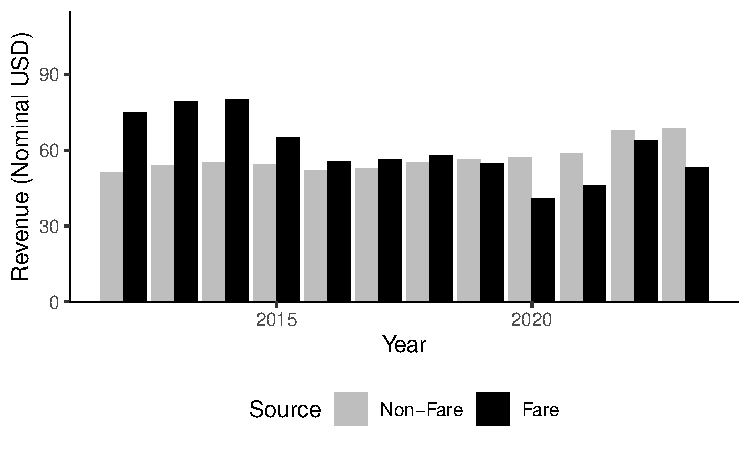
\includegraphics[width = \linewidth]{05.Figures/Spirit_Revenue_Sources.pdf}
\footnotesize{Source: Spirit Airlines 10-K Filings. Values are average revenue per passenger flight segment in nominal dollars. }
\end{figure}

\begin{figure}[h]
\caption{Quarterly Passengers, JetBlue and Spirit}
\label{fig:Quarterly_Pass_JB_SP}
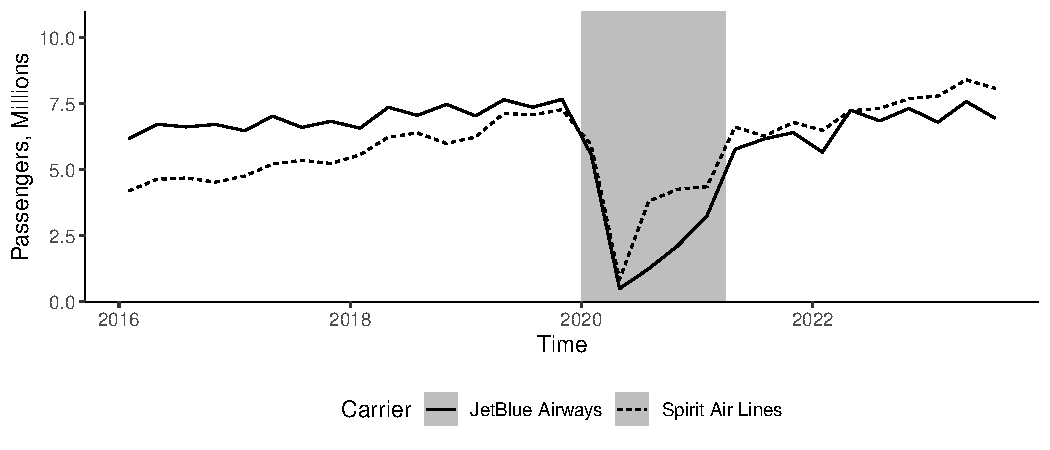
\includegraphics[width = \linewidth]{Spirit_JetBlue_Ridership.pdf}
\footnotesize{Source: DB1B Data. Shaded region depicts the duration of the coronavirus pandemic before widespread vaccine availability within the United States, namely, from the first quarter of 2020 through the first quarter of 2021.}
\end{figure}

\begin{figure}[h]
	\caption{JetBlue, Spirit Fleet Size Over Time}
	\label{fig:Both_fleet}
	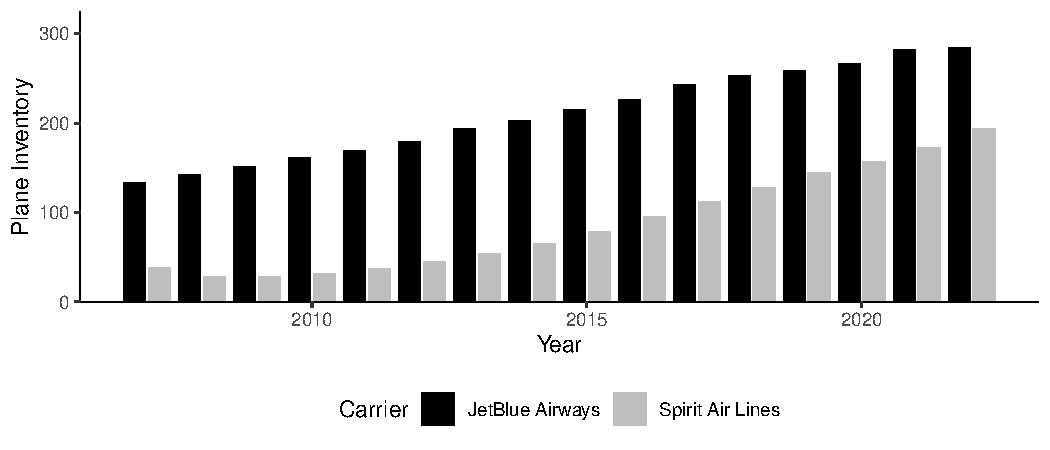
\includegraphics[width = \linewidth]{Both_Planes.pdf}
	\footnotesize{Source: B-43 Inventory Data. Each bar is the number of airplanes in a given firm's inventory within a given year.}
\end{figure}

\begin{figure}
	\caption{JetBlue, Spirit Airports - 2022}
	\label{fig:JBSpirit_Airports_2022}
	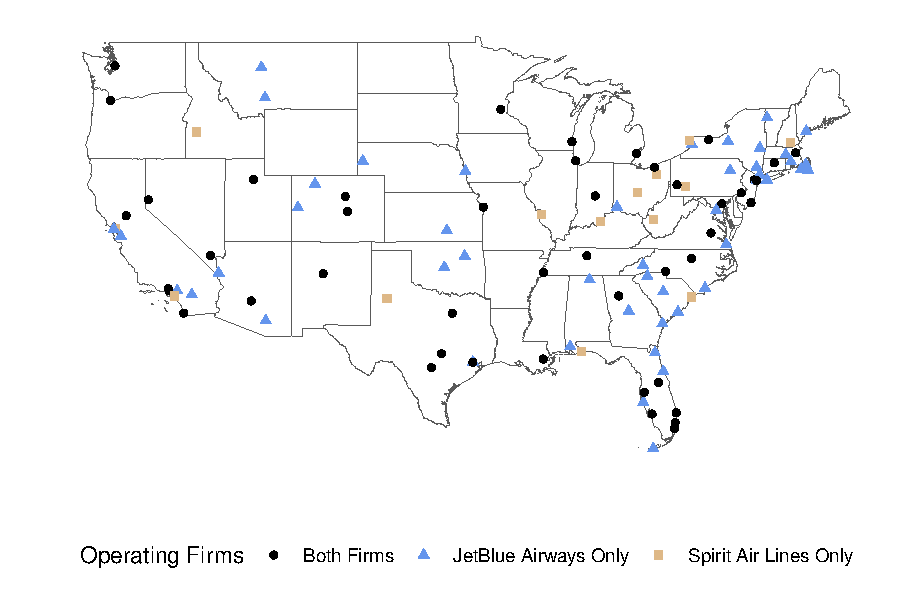
\includegraphics[width = \linewidth]{Map_Mainland_Both_2022.pdf}
	\footnotesize{Derived from DB1B Data. Beyond the United States mainland, both carriers operated in Puerto Rico.}
\end{figure}

\begin{figure}[h]
        \caption{Distribution of Low-Cost and Ultra-Low-Cost Carriers}
        \label{fig:LCC_Distribution}
        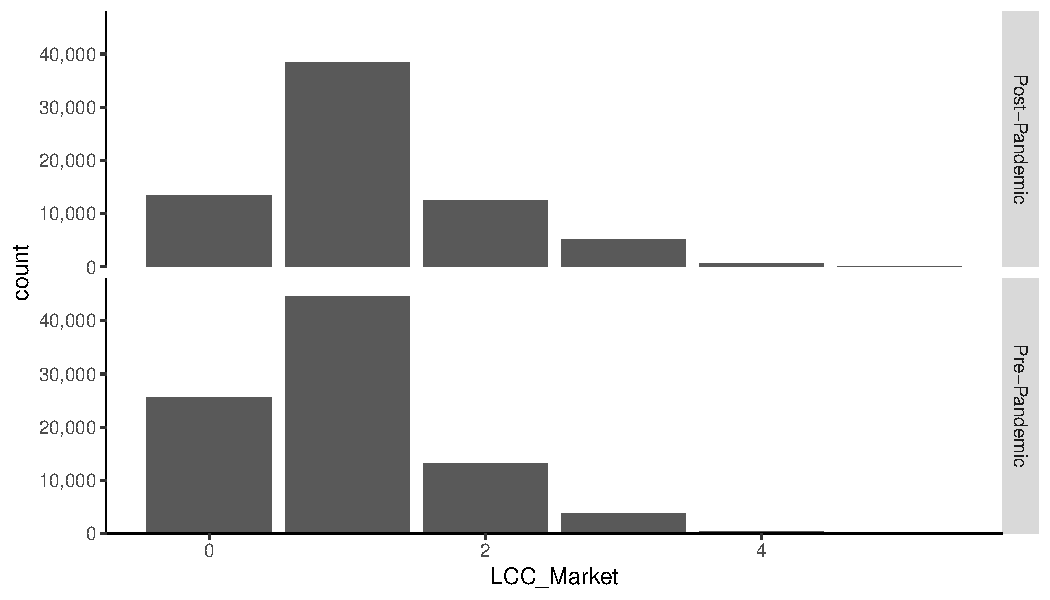
\includegraphics[width = \linewidth]{05.Figures/LCC_Market_Graph.pdf}
        \footnotesize{Derived from the sample with construction methodology described in Appendix \ref{sec:DataProcessing}. Each market is a Year-Quarter-Origin Airport-Destination Airport ordered quartet. Carriers included in the count of low-cost and ultra-low-cost carriers are Southwest, JetBlue, Spirit, Frontier, and Allegiant.}
    \end{figure}

\begin{figure}[h]
	\caption{Quarterly Passengers, All Carriers}
	\label{fig:QuarterlyPass}
	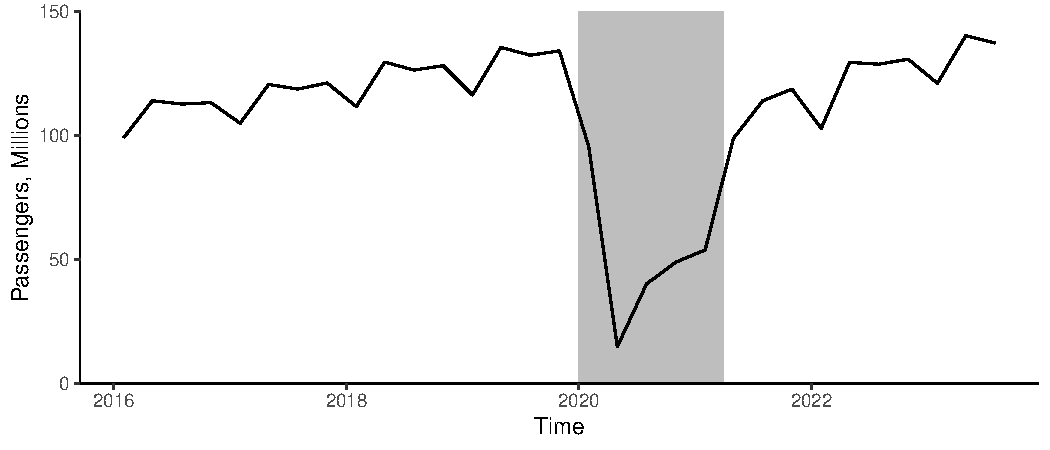
\includegraphics[width = \linewidth]{Quarterly_DB1B_Itineraries}
	\footnotesize{Source: DB1B Data. Shaded region depicts the duration of the coronavirus pandemic before widespread vaccine availability within the United States, namely, from the first quarter of 2020 through the first quarter of 2021.}
\end{figure}
    
      \begin{figure}
    \caption{Simulated Change in Pre-Pandemic Minimum Market Fares}
    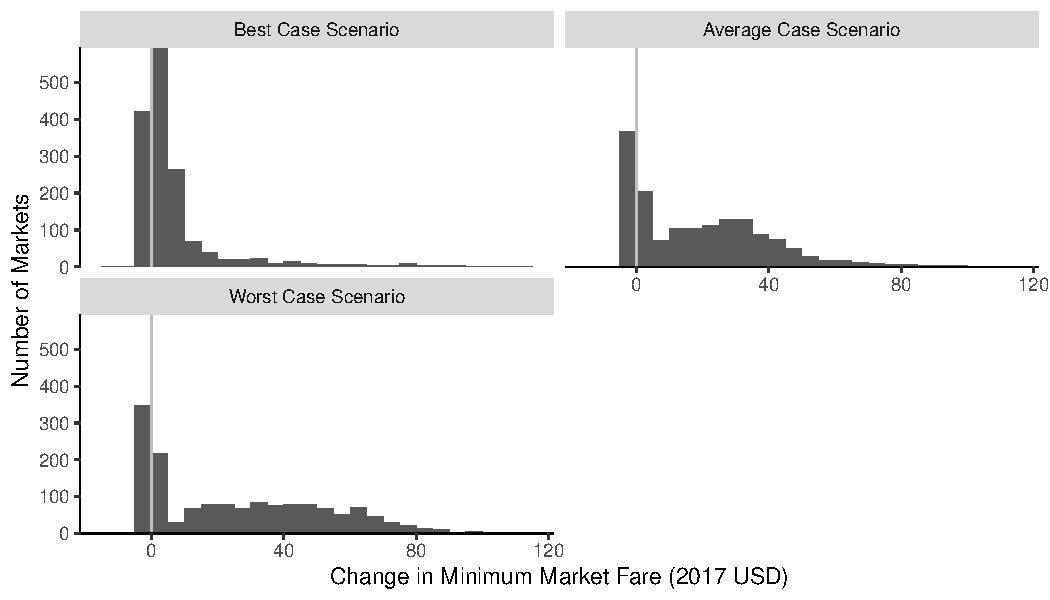
\includegraphics[width = \linewidth]{PrePandemic_Merger_Change_MinimumFare_Dist}
    \label{fig:PrePan_MinimumFare_Dist}
    \footnotesize{The mean change in markets' minimum fares is \$7.25 (\$19.36) [\$26.15] in the best (average) [worst] case merger simulations respectively. Products from markets without both JetBlue and Spirit present are excluded. The best case merger scenario is one in which the combined firm inherits the minimum average cost and greatest unobservables of each firm, the average case merger scenario has the combined JetBlue-Spirit inherit the average of the two firms' product characteristics, and the worst case scenario has the combined JetBlue-Spirit inherit the greatest marginal cost and lowest unobserveables. Prices are in 2017 dollars.}  
    \end{figure}    

    \begin{figure}
    \caption{Simulated Change in Post-Pandemic Minimum Market Fares}
    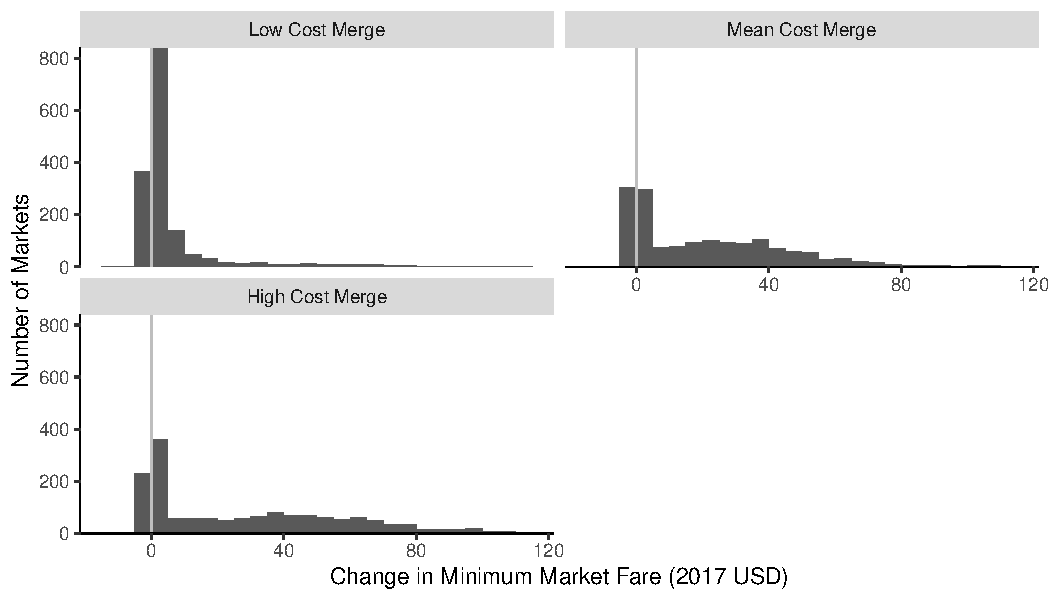
\includegraphics[width = \linewidth]{Merger_Change_MinimumFare_Dist}
    \label{fig:PostPan_MinimumFare_Dist}
    \footnotesize{The mean change in markets' minimum fares is \$6.51 (\$21.45) [\$29.21] in the best (average) [worst] case merger simulations respectively. Products from markets without both JetBlue and Spirit present are excluded. The best case merger scenario is one in which the combined firm inherits the minimum average cost and greatest unobservables of each firm, the average case merger scenario has the combined JetBlue-Spirit inherit the average of the two firms' product characteristics, and the worst case scenario has the combined JetBlue-Spirit inherit the greatest marginal cost and lowest unobserveables. Prices are in 2017 dollars.}
    \end{figure}    

    
    \begin{figure}
        \caption{Distribution in Changes of Average Market Fare - Pre-Pandemic}
        \label{fig:AverageFare_ChangeDist_PrePandemic}
        \begin{center}
        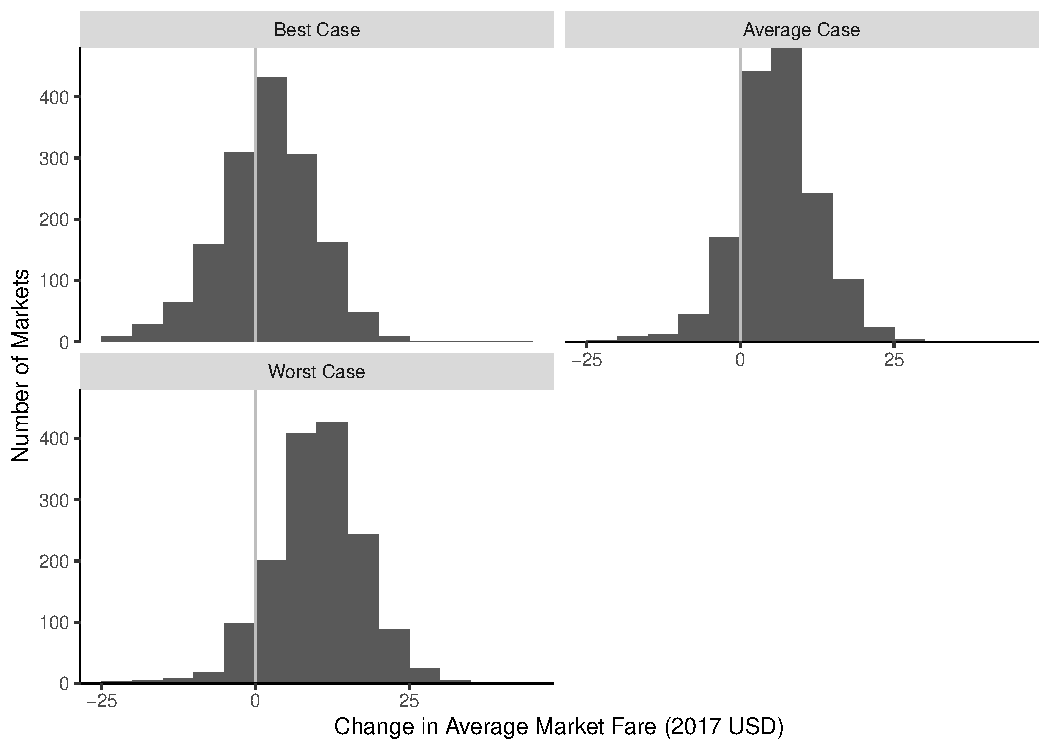
\includegraphics[width = \linewidth]{PrePandemic_Merger_Change_AverageFare_Dist.pdf}
        \end{center}
        \footnotesize{The mean change in markets' average fares is \$2.81 (\$7.46) [\$12.27] in the best (average) [worst] case merger simulations respectively. Products from markets without both JetBlue and Spirit present are excluded. The best case merger scenario is one in which the combined firm inherits the minimum average cost and greatest unobservables of each firm, the average case merger scenario has the combined JetBlue-Spirit inherit the average of the two firms' product characteristics, and the worst case scenario has the combined JetBlue-Spirit inherit the greatest marginal cost and lowest unobserveables. Prices are in 2017 dollars.}     

    \end{figure}

    \begin{figure}
        \caption{Distribution in Changes of Average Market Fare - Post-Pandemic}
        \label{fig:AverageFare_ChangeDist_PostPandemic}
        \begin{center}
        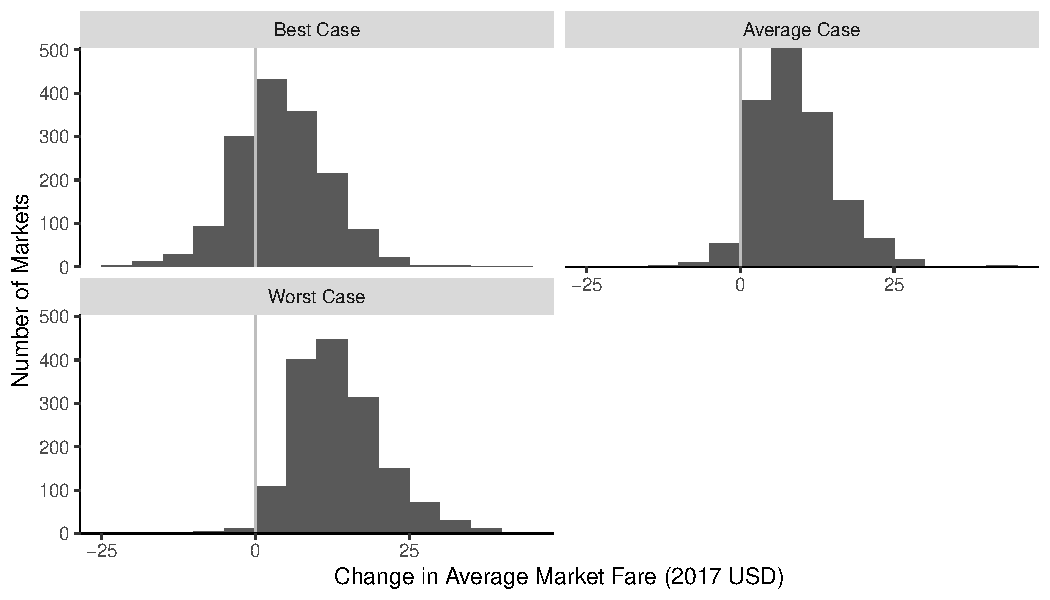
\includegraphics[width = \linewidth]{Merger_Change_AverageFare_Dist.pdf}
        \end{center}
            \footnotesize{The mean change in markets' average fares is \$4.08 (\$8.78) [\$13.64] in the best (average) [worst] case merger simulations respectively. Products from markets without both JetBlue and Spirit present are excluded. The best case merger scenario is one in which the combined firm inherits the minimum average cost and greatest unobservables of each firm, the average case merger scenario has the combined JetBlue-Spirit inherit the average of the two firms' product characteristics, and the worst case scenario has the combined JetBlue-Spirit inherit the greatest marginal cost and lowest unobserveables. Prices are in 2017 dollars.}     
    \end{figure}


    \begin{figure}
        \caption{Change in Estimated Marginal Cost (Percent, Pre-Pandemic)}
        \label{tab:Fee_Fix_prepandemic_MC_PercentChange}
        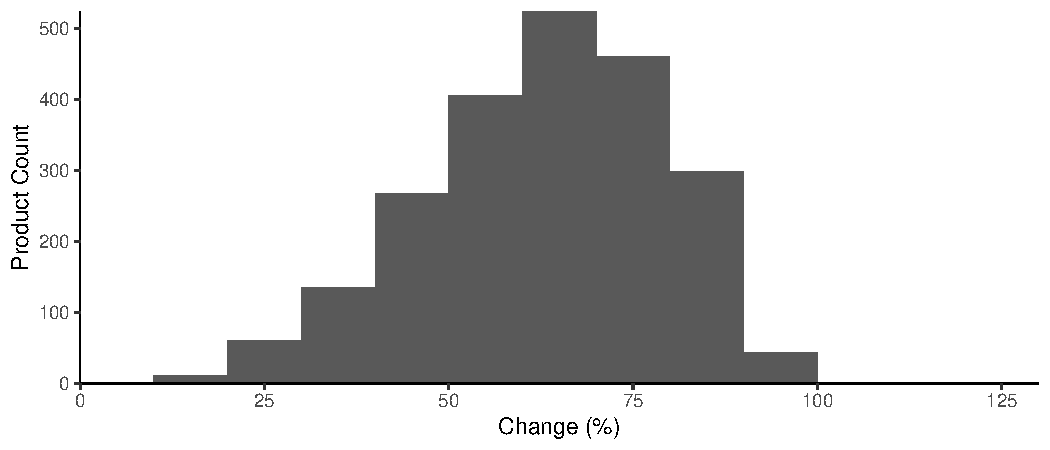
\includegraphics[width = \linewidth]{Fee_Fix_prepandemic_MC_Graph_Percent_JBMarket.pdf}
        \footnotesize{For each Spirit product offered in a post-pandemic market that JetBlue competed against Spirit within, this figure records the change in the estimated marginal cost between the model using the reported fares from the DB1B and the model using the adjusted fares to attempt to capture the impact of ancillary fees on Spirit's total prices. The mean increase in estimated marginal costs is 62.9 percent.}
    \end{figure}
    

    \begin{figure}
        \caption{Change in Estimated Marginal Cost (Percent, Post-Pandemic)}
        \label{tab:Fee_Fix_postpandemic_MC_PercentChange}
        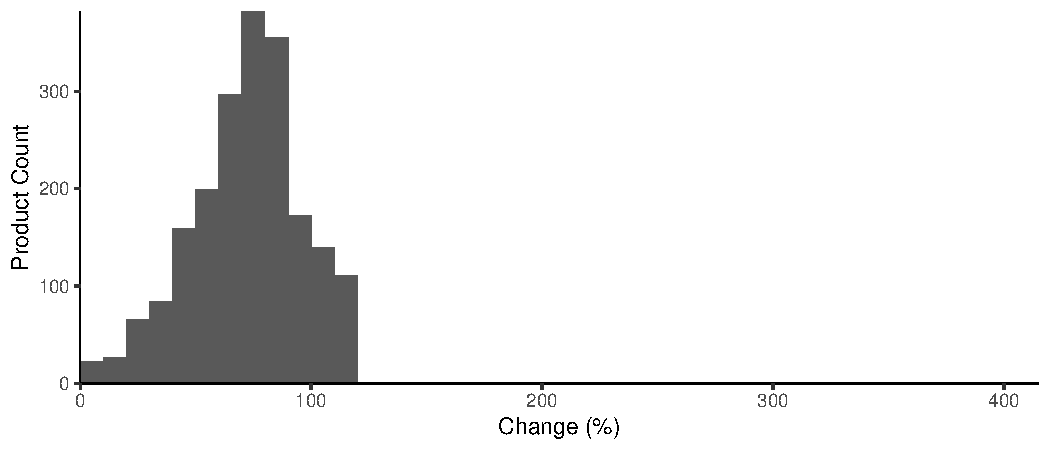
\includegraphics[width = \linewidth]{Fee_Fix_MC_Graph_Percent_JBMarket.pdf}
        \footnotesize{For each Spirit product offered in a post-pandemic market that JetBlue competed against Spirit within, this figure records the change in the estimated marginal cost between the model using the reported fares from the DB1B and the model using the adjusted fares to attempt to capture the impact of ancillary fees on Spirit's total prices. The mean increase in estimated marginal costs is 64.2 percent.}
    \end{figure}  

\FloatBarrier
\pagebreak
\begin{appendices}
    
\setcounter{table}{0}
\setcounter{figure}{0}
\renewcommand{\thetable}{\Alph{section}\arabic{table}}
\renewcommand{\thefigure}{\Alph{section}\arabic{figure}}

	\section{Data Processing Methodology}
	\label{sec:DataProcessing}
	As detailed in Section \ref{sec:Data},	I used the the Bureau of Transportation Statistics' Airline Origin and Destination Survey (DB1B) database as the primary data source for this paper. After compiling the DB1B into a single dataset for the years 2017 through the second quarter of 2023, I excluded observations from my sample using common criteria from the literature. Itineraries with fares lower than \$15 were excluded to remove air travel purchased through frequent flier rewards points (4.88\% of itineraries were excluded this way). Similarly, in line with prior work such as \citet{berry_tracing_2010}, itineraries with reported fares of over \$2,000 dollars were excluded to avoid erroneously recorded fares (0.08\% of itineraries were excluded this way). Beyond fares, itineraries were excluded from the sample if they had three or more layovers\footnote{A total of 0.03\% of itineraries were excluded this way.} or if they had a leg outside of the continental United States.\footnote{As noted in \citet{ciliberto_market_2021}, these flights receive subsidies from the United States Postal Service. As such, proper marginal cost recovery is infeasible while including them in the sample.} 
	
	I additionally excluded products and markets on the basis of several criteria. All markets within the year 2020 and the first quarter of 2021 were dropped to avoid capturing the decline in travel caused by the pandemic which is depicted in Figure \ref{fig:QuarterlyPass}. Furthermore, markets were excluded if they had fewer than 500 passengers fly within them, or had origin and destination airports within 150 miles. This restriction is in line with the past-literature (such as \citet{ciliberto_does_2014}) and serves to not only improve computational speed but also account for these markets featuring stronger substitutability to the outside good for travel. I excluded .0039 of all JetBlue passengers and 0.0020 of all Spirit passengers with the market size criterion. Furthermore, I excluded 0.002 of all JetBlue passengers and under one-ten thousandth of all Spirit passengers with the distance restriction. As such, I view it as unlikely that these criterion significantly changed my results as they apply to the proposed JetBlue-Spirit merger.
    
    Furthermore, to improve computational speed, I drop all markets with origin or destination outside of the 100 largest metropolitan statistical areas in the United States by population. This decision is notably unlikely to significantly impact the results of this paper as both JetBlue and Spirit focus their operations on larger metropolitan statistical areas. Finally, I exclude products with fewer than 100 passengers were excluded from the sample to avoid capturing irregular product offerings (2.50\% of itineraries were excluded this way). 
    	
	In calculating product shares, I estimate the total number of passengers of each product as being ten times the number of passengers recorded as purchasing it within the DB1B. I do this as the DB1B is a 10\% sample of airline itineraries. Then, I divide each ridership estimate by the geometric mean of the origin and destination metropolitan areas, in line with the past literature. 
	
	% Beyond the handling of data acquired from the DB1B, data on the daily spot price of jet fuel was acquired through the U.S. Energy Information Administration. This was averaged at the quarterly level. 
	
	As part of the handling of price data, I modify prices in two ways. For Spirit itineraries completed before 2020, fares had an additional \$22.99 times the number of trip legs added to them to accounts for Spirit's additional usage fee placed on itineraries which were not booked in-person at the airport. As noted in \citet{shrago_spirit_2024}, the majority of Spirit's customers paid these fees and these fees were included in the base ticket price in DB1B releases following 2020. Furthermore, I re-express prices in terms of 2017 United States dollars to allow for easier comparisons between the two sample periods due to the high levels of inflation within the post-pandemic period.

    \FloatBarrier
    
    \section{Northeast Alliance}
	\label{sec:Setting_NEA}
	
	Prior to its attempted merger with Spirit, JetBlue entered into the Northeast Alliance (NEA) with American Airlines at the start of 2021. The NEA saw the two firms coordinate operations to behave as a single carrier for routes that touched upon airports serving the New York City and Boston markets. They jointly decided their network for these routes, and operated them intending for consumers to be indifferent between the two carriers, worked to minimize overlap in product offerings on these routes, and shared revenue from products within the agreement. The United States Department of Justice along with six states and the District of Columbia brought a lawsuit against the agreement in September 2021 alleging violations of the Sherman Antitrust Act. Following a 2022 trial, the agreement would be found to violate the Sherman Antitrust Act in May 2023 and it was subsequently unwound \citep{rennison_jetblue-american_2023, rains_what_2023}.\footnote{Table \ref{tab:NEA_Timeline} details a timeline of key events relating to the NEA. Notably, some landing slot leases between the two airlines related to the merger experienced a gradual reversion to their original owners.} With this timeline outlined, I will briefly discuss the NEA's differences from traditional airline alliances and the issues it presents for the estimation of the counterfactual merger effects of the JetBlue-Spirit merger. 

    \begin{table}[tb]
		\caption{Northeast Alliance Timeline}
		\label{tab:NEA_Timeline}
		\begin{center}
			\begin{tabular}{ccc}
				\hline
				Year & Date & Event \\
				\hline
				2020 & Quarter 1-2 & JetBlue and American Negotiate Alliance \\ 
				& July 16 & Northeast Alliance Announced \\
				& July 22 & Alliance Agreement submitted to DOT \\
				\hline 
				2021 & January 10 & DOT Terminates Antitrust Review \\
				& February 24 & Codesharing Agreement Begins on {X} Routes \\
				& May 26 & Reciprocal Loyalty Earnings Begins \\
				& Early September & NEA Shuttle at JFK Opens \\
				& September 21 & DOJ Files Lawsuit Against NEA \\  
				\hline
				2022 & September 27 - November 18 & Trial \\
				\hline 
				2023 & May 19 & NEA Ruled Anti-Competitive \\
				& July 5 & JetBlue Drops Appeal Plans \\
				& July 21 & NEA Codesharing Ends \\
				& October 31 & JFK Shuttle Ceases Operation\\
				& October 31 & 12 Slot Leases to JetBlue Terminate \\
				\hline 
				2024 &  March 31  & 27 Slot Leases to JetBlue Terminate \\ 
				& March 31 & 1 Slot Lease to American Terminates \\
				& October 26 & Remaining NEA Slot Leases Terminate				 \end{tabular}
		\end{center}
	\end{table}

	Alliances between airlines are commonplace within the industry. Two prominent examples of these alliances are the ``SkyTeam Alliance" (which includes Delta) and the ``Star Alliance" which includes United. One key feature of these alliances are code-sharing agreements which allow member firms to sell seats on flights operated by other members of the alliances. Alliances are primarily operated between carriers situated in different countries to allow for better access to foreign markets than would otherwise be possible. Alliances benefit consumers through the increased ability to earn frequent flier miles, easier handling of baggage, and simpler booking processes. Meanwhile, alliances benefit airlines through allowing them to offer travel to a wider variety of destinations than would otherwise be possible without participation in an alliance. 
	
	Domestic alliances are presently rare. Unlike alliances between domestic and foreign carriers, these agreements are generally unable to receive waivers from antitrust proceedings through the Department of Transportation and as such face additional regulatory scrutiny. One common way for firms to operate domestic alliances is by structuring the agreement to only cover markets without both firms and by requiring that member firms otherwise maintain separate routing decisions, operations, and planning. One example of a currently active domestic airline alliance is the West Coast Alliance between American and Alaska Airlines.  
	
	Contrasting this approach, the NEA was structured to act more similarly to a merger on routes covered by the agreement. The two firms jointly scheduled flights within the impacted markets, minimized overlap on routes operated by both firms\footnote{It is not clear how effective this was. As documented in Figure \ref{fig:NEA_Operating}, the levels of shared routes at each of the four impacted airports was within historically normal ranges.}, and coordinated operations at the airports impacted by the agreement.\footnote{One example of this coordination is a shuttle operated by the two airlines at JFK to allow customers to transfer between the terminals used by each airline without having to clear security on connecting itineraries \citep{griff_riding_2021}.} Furthermore, as two of the impacted airports featured slot and gate controls\footnote{A slot-controlled airport is one in which airlines are assigned specified time slots by the FAA for departures and arrivals to allow for better coordination of runway usage in congested airports. These slots are set in advance of individual operation days and can be transferred between airlines as if they were property of the airline which holds them.}, the member firms shared slot permits and shared gates. This would be found by the trial court to have increased barriers to entering the New York City air travel market by deterring these firms by selling off these assets to other firms. 
    
    The NEA impacts the evaluation of the counterfactual effects of the JetBlue-Spirit merger through its effects on the product offerings of JetBlue. Through jointly optimizing its network structure with American Airlines, JetBlue operated flights in different markets than it otherwise would have. As my simulation of the JetBlue-Spirit merger treats product offerings as exogenous, my post-pandemic results should be understood as estimating the world where the merger took place while the NEA was still in effect. 

    Beyond the changes to market structures, the NEA results in products within my sample that are considered JetBlue products despite being operated solely by or jointly with American. The majority of the NEA's existence saw over thirty products a quarter that fits these characteristics within markets both JetBlue and Spirit competed within (Table \ref{tab:NEA_Codesharing_Table}. As such, the recovery of marginal costs for these products is liable to be incorrect.
    

\begin{table}[h]
		\caption{American, JetBlue Overlap at NEA Airports}
		\label{tab:NEA_Airport_Presence}
        \vspace{-15mm}
        \begin{center}
         
\begin{tabular}[t]{rrrrrrrrr}
\toprule
\multicolumn{1}{c}{ } & \multicolumn{2}{c}{JFK} & \multicolumn{2}{c}{BOS} & \multicolumn{2}{c}{LGA} & \multicolumn{2}{c}{EWR} \\
\cmidrule(l{3pt}r{3pt}){2-3} \cmidrule(l{3pt}r{3pt}){4-5} \cmidrule(l{3pt}r{3pt}){6-7} \cmidrule(l{3pt}r{3pt}){8-9}
Year & Ticket & Operating & Ticket & Operating & Ticket & Operating & Ticket & Operating\\
\midrule
\addlinespace[0.3em]
\multicolumn{9}{l}{\textbf{Q1}}\\
\hspace{1em}2023 & 75.4 & 23.7 & 69.1 & 21.4 & 67.3 & 4.2 & 46.7 & 7.7\\
\hspace{1em}2022 & 77.0 & 29.7 & 75.0 & 29.1 & 73.9 & 8.9 & 47.6 & 8.3\\
\hspace{1em}2021 & 18.6 & 24.4 & 26.8 & 21.7 & 50.0 & 33.3 & 9.5 & 13.6\\
\hspace{1em}2019 & 22.4 & 23.3 & 22.9 & 20.0 & 8.1 & 6.7 & 0.0 & 0.0\\
\addlinespace[0.3em]
\multicolumn{9}{l}{\textbf{Q2}}\\
\hspace{1em}2023 & 70.0 & 15.9 & 63.1 & 22.2 & 68.3 & 5.4 & 46.7 & 7.7\\
\hspace{1em}2022 & 68.3 & 26.5 & 70.3 & 21.9 & 75.0 & 6.4 & 45.5 & 17.4\\
\hspace{1em}2021 & 57.7 & 21.1 & 57.4 & 28.6 & 27.3 & 7.4 & 28.6 & 13.6\\
\hspace{1em}2019 & 21.1 & 21.0 & 21.2 & 25.0 & 8.9 & 5.6 & 0.0 & 0.0\\
\addlinespace[0.3em]
\multicolumn{9}{l}{\textbf{Q3}}\\
\hspace{1em}2023 & 69.0 & 16.9 & 63.9 & 19.0 & 61.0 & 4.1 & 40.0 & 7.7\\
\hspace{1em}2022 & 73.8 & 21.9 & 73.8 & 24.2 & 75.9 & 6.4 & 57.1 & 7.1\\
\hspace{1em}2021 & 63.6 & 25.9 & 58.9 & 23.1 & 30.4 & 3.2 & 37.5 & 14.8\\
\hspace{1em}2019 & 19.6 & 20.3 & 21.6 & 21.6 & 8.9 & 5.6 & 0.0 & 0.0\\
\addlinespace[0.3em]
\multicolumn{9}{l}{\textbf{Q4}}\\
\hspace{1em}2022 & 72.1 & 25.4 & 66.1 & 21.1 & 69.8 & 2.0 & 46.7 & 7.7\\
\hspace{1em}2021 & 71.9 & 25.8 & 73.2 & 23.2 & 75.0 & 4.3 & 43.5 & 7.7\\
\hspace{1em}2019 & 15.3 & 17.5 & 22.0 & 19.2 & 6.8 & 5.4 & 0.0 & 0.0\\
\bottomrule
\end{tabular}

        \end{center}
                \vspace{-5mm}
		\footnotesize{Each cell is the percent of markets originating from the specified airport with both carriers present in the market as either the ticketing carrier or operating carrier. Ticketing carriers are responsible for buying and selling of tickets while the operating carrier handles flight operations. Data for the first quarter of 2021 should be interpreted cautiously as this was before widespread vaccination availability.}
\end{table}


    \begin{figure}
        \caption{Northeast Alliance Passenger Uptake}
        \label{fig:NEA_Uptake}
        \begin{center}
        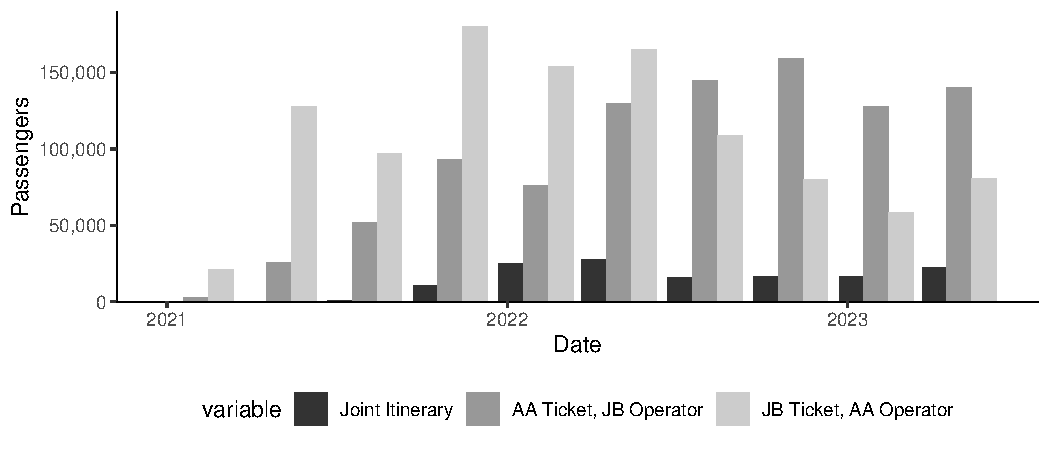
\includegraphics[width = \linewidth]{05.Figures/NEA_OperationsGraph}
        \end{center}
        \vspace{-8mm}
        \footnotesize{A joint itinerary is one in which both JetBlue and American Airlines operated flights on one or more legs of the unidirectional trip. The ticketing carrier collects fares and issues tickets, the operating carrier operates the flights. Itineraries are classified as an "AA Ticket, JB Operator" if the entire itinerary was issued by American Airlines and JetBlue operated at least one leg of the trip.}
    \end{figure}

\begin{landscape}
    \begin{table}
        \caption{NEA Codesharing Products}
        \label{tab:NEA_Codesharing_Table}
        \vspace{-15mm}
        \begin{center}
        
\begin{tabular}[t]{lrrrrrrrrrrr}
\toprule
 & 2021Q1 & 2021Q2 & 2021Q3 & 2021Q4 & 2022Q1 & 2022Q2 & 2022Q3 & 2022Q4 & 2023Q1 & 2023Q2 & 2023Q3\\
\midrule
\addlinespace[0.3em]
\multicolumn{12}{l}{\textbf{All Markets}}\\
\hspace{1em}JetBlue Only & 843 & 1375 & 1327 & 1374 & 1363 & 1583 & 1531 & 1456 & 1412 & 1562 & 1640\\
\hspace{1em}JetBlue American Required & 10 & 22 & 25 & 17 & 24 & 27 & 21 & 29 & 18 & 41 & 35\\
\hspace{1em}JetBlue-American Joint & 0 & 0 & 0 & 67 & 90 & 69 & 50 & 85 & 74 & 134 & 90\\
\hspace{1em}American Only & 4487 & 6728 & 7534 & 7351 & 7119 & 7596 & 8099 & 8338 & 7742 & 8173 & 8434\\
\hspace{1em}American JetBlue Required & 61 & 90 & 86 & 87 & 84 & 88 & 87 & 75 & 81 & 81 & 86\\
\hspace{1em}American-JetBlue Joint & 1 & 0 & 0 & 1 & 0 & 0 & 2 & 1 & 2 & 6 & 3\\
\addlinespace[0.3em]
\multicolumn{12}{l}{\textbf{Spirit Markets}}\\
\hspace{1em}JetBlue Only & 338 & 438 & 420 & 447 & 409 & 517 & 490 & 540 & 554 & 644 & 676\\
\hspace{1em}JetBlue American Required & 4 & 11 & 6 & 9 & 10 & 15 & 12 & 14 & 11 & 17 & 12\\
\hspace{1em}JetBlue-American Joint & 0 & 0 & 0 & 22 & 26 & 20 & 16 & 27 & 25 & 44 & 33\\
\hspace{1em}American Only & 1161 & 1491 & 1694 & 1849 & 1773 & 2012 & 2112 & 2340 & 2309 & 2563 & 2666\\
\hspace{1em}American JetBlue Required & 16 & 28 & 28 & 30 & 27 & 31 & 16 & 23 & 21 & 25 & 28\\
\hspace{1em}American-JetBlue Joint & 0 & 0 & 0 & 0 & 0 & 0 & 0 & 0 & 0 & 0 & 1\\
\bottomrule
\end{tabular}

        \end{center}
        \vspace{-5mm}
        \footnotesize{Each row indicates the number of products within a given quarter that belong to each classification. A "Firm Only" product is one in which the product had no codesharing flights included within it. A "JetBlue American Required" product is one in which all itineraries credited to the JetBlue for that quarter had all legs operated by American. A "JetBlue-American Joint" product is one where at least one leg was operated by each firm. A Spirit Market is one in which Spirit operated within it during the given quarter of interest. }
    \end{table}
\end{landscape}
    \begin{figure}[h]
        \caption{NEA: Overlapped Operating Routes}
        \label{fig:NEA_Operating}
        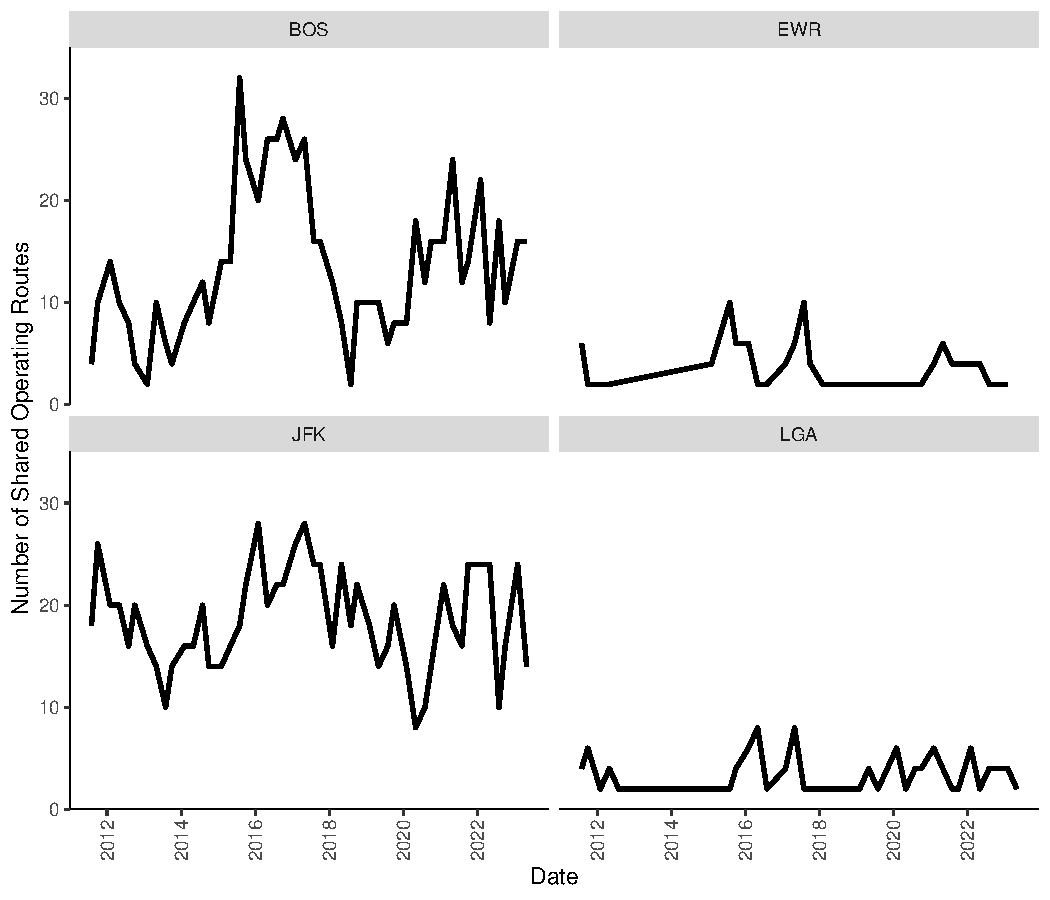
\includegraphics[width = \linewidth]{05.Figures/NEA_Operating_Graph.pdf}
        \footnotesize{Figure plots the number of routes operated by both JetBlue and American within a given quarter. The vertical line represents the start of the Northeast Alliance in January 2021.}
    \end{figure}
    \FloatBarrier
    \section{Merger Announcement Effects}
    \setcounter{table}{0}
    \setcounter{figure}{0}

    Historically, airline mergers have had effects on airfares before the completion of the merger. Within this section, I estimate the effects of the announcement of the merger on fares in markets served by both JetBlue and Spirit through a modified version of the event study model used in \citet{goolsbee_how_2008} and \citet{fan_when_2020}. I use an alternative subsample of the data I use within the main text consisting of route-period-carrier level observations of the log average-fare offered by each carrier within two types of markets - those consistently served by both JetBlue and Spirit in the four quarters prior to the merger announcement and markets in which JetBlue and Spirit did not fly within the four quarters prior to the merger announcement. I further restrict this sample to only include markets after the first quarter of 2021. 
    
    For carrier $c$ serving unidirectional route $r$ at time $t$, its log-average fare $y_{crq}$ is described by 

    \[y_{crt} = Merge_{r} \sum_{i = - 4, i \neq -1}^{4} \beta_{i}I[t = i]  + \mu_{cr} + \mu_{t} + \epsilon_{crt}\]

    where $I[q = i]$ is $1$ if $q = i$ and zero otherwise, $Merge_{c}$ is a dummy variable which is one if both JetBlue and Spirit operate within the market, $Other_c$ is one if the carrier neither of the merging firms, $\mu_{cr}$ is vector containing fixed effects for both carrier and route, $X_{crq}$ is a vector of controls, and $\epsilon_{crq}$ is a random error term. As the Spirit-JetBlue merger was approved by Spirit's board in the third quarter of 2022, period $0$ is defined as the second quarter of 2022. Furthermore, quarters from the height of the coronavirus pandemic (2020 and the first quarter of 2021) are excluded. 

    As documented in Figure \ref{fig:MergerAnnouncement_Plot}, I fail to find evidence for significant anticipatory effects caused by the JetBlue-Spirit merger. I hypothesize that this may be due to the lower market share of these two firms in comparison to the previous literature which found anticipatory effects caused by the mergers of legacy airlines. 

    \begin{figure}
    \caption{Merger Announcement Event Study}
    \label{fig:MergerAnnouncement_Plot}
    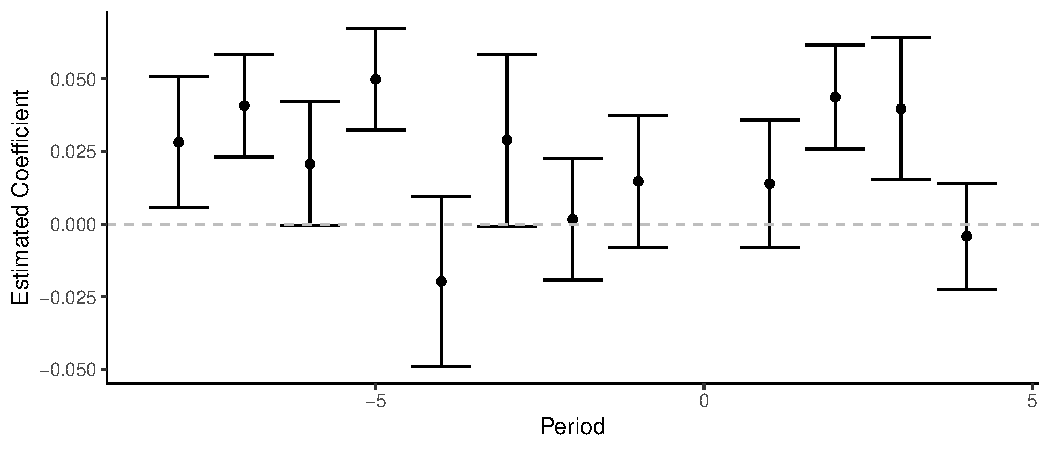
\includegraphics[width = \linewidth]{05.Figures/Merger_Anticipate_Figure.pdf}
    \end{figure}

    \FloatBarrier
	\section{Merger Comments Analysis}
    \label{sec:NaturalLanguage}

    \setcounter{table}{0}
    \setcounter{figure}{0}


As part of the merger process, JetBlue and Spirit were required to file an application with the Department of Transportation for the transference of operating certificates from Spirit to the combined firm, effective after the completion of the merger. Members of the public were allowed to leave public comments on the regulatory filing. Within this section, I employ stance detection techniques to analyze these comments at scale. While these comments are largely irrelevant to the ultimate blocking of the merger (namely, that it would be rejected following a suit brought by the Department of Justice), Spirit and JetBlue used these comments as part of their attempt gain public approval for the merger.

Stance detection is the task of detecting the position held by the author of a text regarding some topic. In this context, it is to determine if the author of a comment left on the regulatory filing supported or opposed the proposed JetBlue-Spirit merger. This context is particularly suitable for the use of modern machine learning models as these comments are focused (the econometrician knows the topic of the comments) and limited in length (larger bodies of text are unsuitable for the methodology used within this section). As such, I believe that an unsupervised pre-trained model should be effective at trying to gauge the stance of these comments. 

The stance detection problem should not be confused with that of the sentiment analysis problem. Sentiment analysis intends to capture the emotions expressed in a text rather than identify the emotions expressed within the text. As an example of how these differ, consider the comment ``Competition is good for a healthy economy."\footnote{This is an actual comment left on the regulatory docket.} Using a pre-trained sentiment detection model developed for analyzing financial sentiment data, FinBERT, \footnote{Model documentation is contained in \citet{araci_finbert_2019}.} this statement is correctly judged to possess positive sentiment (it uses positive language to describe competition). However, the stance detection model I use correctly judges this comment to oppose the merge. Table \ref{tab:Sentiment_Stance_Table} details the breakdown of unique comments' assigned sentiments and stances. 

\begin{table}
    \caption{Sentiment and Stance - Unique Comments}
    \label{tab:Sentiment_Stance_Table}
    \vspace{-15mm}
    \begin{center}
    
\begin{tabular}[t]{llll}
\toprule
\multicolumn{1}{c}{Stance} & \multicolumn{3}{c}{Sentiment} \\
\cmidrule(l{3pt}r{3pt}){1-1} \cmidrule(l{3pt}r{3pt}){2-4}
 & Positive & Neutral & Negative\\
\midrule
Approves & 40 & 37 & 4\\
Disapproves & 5 & 387 & 227\\
\bottomrule
\end{tabular}

    \end{center}
        \vspace{-5mm}
    \footnotesize{Each cell includes the number of comments with the given stance and sentiment. Only unique comments are included within this table. }
\end{table}

This paper uses the pre-trained model documented in \citet{laurer_less_2024} to detect the stances of each comment left on the docket. Each comment is assessed for the probability that each comment agrees with the statements ``The author of this comment \{approves of, disagrees with\} the merger." As these statements are mutually exclusive, the probabilities assigned for each comment sum to 1. As documented in Figure \ref{fig:ProbabilityApprove} and Figure \ref{fig:ProbabilityApprove_Unique}, most comments are strongly polarized, suggesting that the language model had little difficulty in assigning stances to comments. Looking over a sample of fifty unique comments, all are sorted as would be expected based on my understanding of the text. As such, I believe that this model is well suited for analyzing the public comments.  

	\begin{figure}
		\caption{Probability Comments Approve}
		\label{fig:ProbabilityApprove}
        \begin{center}
        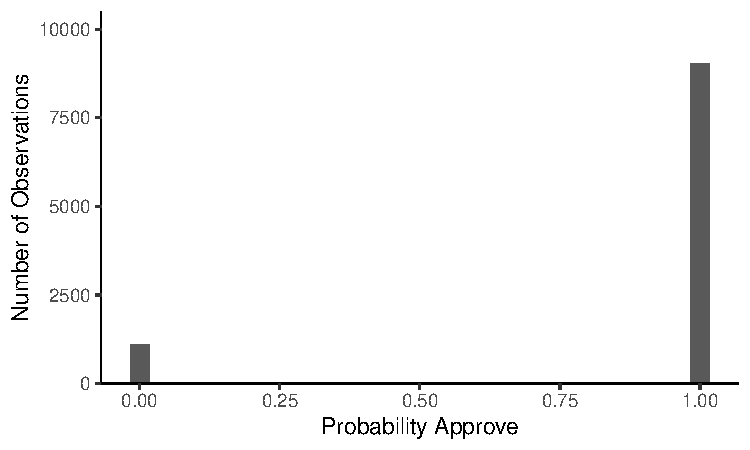
\includegraphics{05.Figures/stance_strength_graph}
        \end{center}
		\begin{minipage}{\textwidth} 
			{\footnotesize Data is sourced from the Department of Transportation regulatory filing regarding the JetBlue-Spirit merger (DOT-OST-2023-0024). ``Probability Approve" is the probability that a comment approves of the merger as asssed by the stance detection model.} 
		\end{minipage}
	\end{figure}
	
	\begin{figure}
		\caption{Probability Comment Approves - Unique Comments Only}
		\label{fig:ProbabilityApprove_Unique}
        \begin{center}
            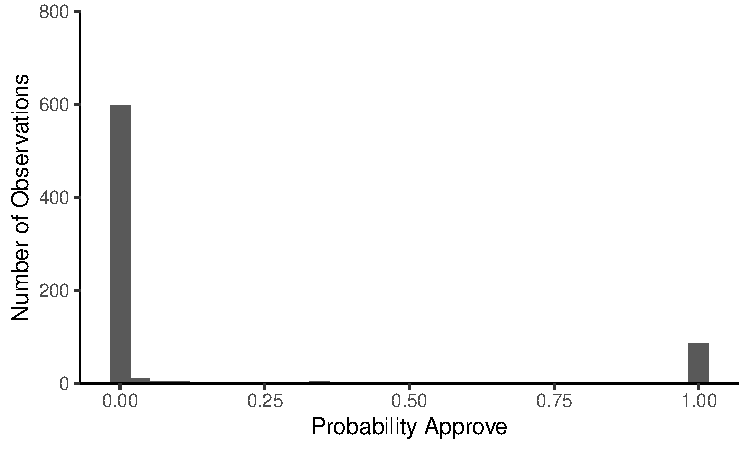
\includegraphics{05.Figures/stance_strength_unique.pdf}
        \end{center}
				\begin{minipage}{\textwidth} 
			{\footnotesize Data is sourced from the Department of Transportation regulatory filing regarding the JetBlue-Spirit merger (DOT-OST-2023-0024). ``Probability Approve" is the probability that a comment approves of the merger as asssed by the stance detection model.} 
		\end{minipage}
	\end{figure}


Table \ref{tab:Stance_Summary} contains summary statistics for these comments. Most comments approve of the merger. However, this is driven by duplicate comments. \footnote{The exact legitimacy of these duplicate comments was a matter of some public debate, with some lawmakers alleging that they represented an "astroturf campaign" by the two merging firms falsely attributing them to employees \citep{birnbaum_elizabeth_2023}.}  The vast majority of unique comments, on the other hand, disapproved of the merger. On average, comments which approve of the merger are longer than those that disapprove. This table provides a helpful demonstration of the difference between the stance detection and sentiment detection problems -  the majority of disapproving comments expressed their views with neutral sentiment. Finally, the table documents the state of origin for the comments. 

\begin{table}[h]
    \caption{Stance Detection Summary Statistics}
    \label{tab:Stance_Summary}
    
\begin{tabular}[t]{llllll}
\toprule
 & Mean & (SD) & Minimum & Median & Maximum\\
\midrule
\addlinespace[0.3em]
\multicolumn{6}{l}{\textbf{All Comments}}\\
\hspace{1em}P(Approves) & 0.89 & (0.31) & 0 & 1 & 1\\
\hspace{1em}Approving Comment P(Approves) & 1 & (0.02) & 0.51 & 1 & 1\\
\hspace{1em}Disapproving Comment P(Approves) & 0.01 & (0.04) & 0 & 0 & 0.49\\
\hspace{1em}New York Comment & 0.14 & (0.35) & 0 & 0 & 1\\
\hspace{1em}Florida Comment & 0.35 & (0.48) & 0 & 0 & 1\\
\hspace{1em}Massachusetts Comment & 0.05 & (0.22) & 0 & 0 & 1\\
\hspace{1em}Puerto Rico Comment & 0.01 & (0.12) & 0 & 0 & 1\\
\midrule
\hspace{1em}Observations & 10185 &  &  &  & \\
\midrule
\addlinespace[0.3em]
\multicolumn{6}{l}{\textbf{Unique Comments}}\\
\hspace{1em}P(Approves) & 0.13 & (0.32) & 0 & 0 & 1\\
\hspace{1em}Approving Comment P(Approves) & 0.98 & (0.08) & 0.51 & 1 & 1\\
\hspace{1em}Disapproving Comment P(Approves) & 0.01 & (0.06) & 0 & 0 & 0.49\\
\hspace{1em}New York Comment & 0.06 & (0.24) & 0 & 0 & 1\\
\hspace{1em}Florida Comment & 0.07 & (0.26) & 0 & 0 & 1\\
\hspace{1em}Massachusetts Comment & 0.03 & (0.18) & 0 & 0 & 1\\
\hspace{1em}Puerto Rico Comment & 0 & (0) & 0 & 0 & 0\\
\midrule
\hspace{1em}Observations & 701 &  &  &  & \\
\midrule
\bottomrule
\end{tabular}

    \begin{minipage}{\textwidth} 
        {\footnotesize Data is sourced from the Department of Transportation regulatory filing regarding the JetBlue-Spirit merger  (DOT-OST-2023-0024). Comments have the stance with the highest probability assigned to them. This is the ``Stance Probability." Similarly, ``Sentiment Assigned Probability" is the sentiment with the highest  probability assigned to a comment by the language model. Comment length is in characters.} 
    \end{minipage}
\end{table}

Figure \ref{fig:CommentTimeline} plots the distribution of submitted comments on each day after the regulation was available for commenting upon. In the first twenty days, virtually every comment left on the docket supported the merger. Virtually every comment left on the docket after this period was opposed the merger. This may reflect asymmetry in the the resources available to JetBlue, Spirit, and anti-merger consumer welfare organizations.  

    \begin{figure}[h]
		\caption{Timeline of Submitted Comments}
		\label{fig:CommentTimeline}
        \begin{center}
    	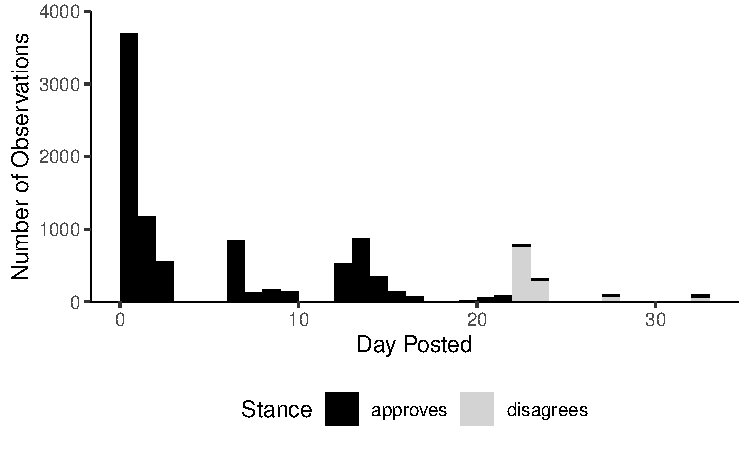
\includegraphics{stance_submission_timeline}
        \end{center}
		\begin{minipage}{\textwidth} 
			{\footnotesize Data is sourced from the Department of Transportation regulatory filing regarding the JetBlue-Spirit merger  (DOT-OST-2023-0024). Comments have the stance with the highest probability assigned to them.} 
		\end{minipage}
	\end{figure}
	    

    \pagebreak 

    \FloatBarrier
    \section{Robustness Checks}
    \setcounter{table}{0}
    \setcounter{figure}{0}
    \subsection{Assumed Merger Efficiencies}
    \label{App:Efficiencies}
    In this section, I consider an alternative simulation method where for each case identified in the main text (Section \ref{sec:Analysis_Merger}), I additionally assume that the merged firm realizes efficiencies of either 5\% or 10\%. The results of this simulation for the 5\% case are reported in Table \ref{tab:Simulation_Price_5} and the results for the 10\% case in Table \ref{tab:Simulation_Price_10}. Minimum fare in market changes are reported in Table \ref{tab:MinimumPrice_5} and Table \ref{tab:MinimumPrice_10}. 

        \begin{table}
        \caption{Simulated Price Effects of Merger with 5\% Efficiency Gain - Joint Markets}
        \label{tab:Simulation_Price_5}
                \vspace{-15mm}
        \begin{center}
         
\begin{tabular}[t]{lllllll}
\toprule
 & N & Mean & (SD) & Minimum & Median & Maximum\\
\midrule
\addlinespace[0.3em]
\multicolumn{7}{l}{\textbf{Pre-Pandemic}}\\
\addlinespace[0.3em]
\multicolumn{7}{l}{\textbf{Product Prices (100s, 2017 USD)}}\\
\hspace{1em}\hspace{1em}Observed & 12074 & 2.04 & (0.69) & 0.47 & 1.98 & 4.91\\
\hspace{1em}\hspace{1em}Best Case & 10106 & 2.06 & (0.67) & 0.46 & 2.01 & 5.08\\
\hspace{1em}\hspace{1em}Average Case & 10106 & 2.1 & (0.64) & 0.46 & 2.04 & 5.14\\
\hspace{1em}\hspace{1em}Worst Case & 10106 & 2.15 & (0.64) & 0.48 & 2.08 & 5.13\\
\addlinespace[0.3em]
\multicolumn{7}{l}{\textbf{Market Average Price}}\\
\hspace{1em}\hspace{1em}Observed & 1418 & 2.01 & (0.43) & 0.93 & 1.95 & \vphantom{1} 3.1\\
\hspace{1em}\hspace{1em}Best Case & 1418 & 1.7 & (0.61) & 0.79 & 1.52 & \vphantom{1} 3.44\\
\hspace{1em}\hspace{1em}Average Case & 1418 & 1.97 & (0.51) & 0.99 & 1.88 & \vphantom{1} 3.37\\
\hspace{1em}\hspace{1em}Worst Case & 1418 & 2 & (0.5) & 0.99 & 1.9 & \vphantom{1} 3.49\\
\addlinespace[0.3em]
\multicolumn{7}{l}{\textbf{\% Change Average Price}}\\
\hspace{1em}\hspace{1em}Best Case & 1418 & -16.62 & (17.31) & -54.03 & -18.81 & 31.39\\
\hspace{1em}\hspace{1em}Average Case & 1418 & -2.16 & (10.5) & -40.03 & -2.04 & 38.88\\
\hspace{1em}\hspace{1em}Worst Case & 1418 & -0.71 & (10.38) & -34.5 & -0.51 & 37.08\\
\addlinespace[0.3em]
\multicolumn{7}{l}{\textbf{Median Price}}\\
\hspace{1em}\hspace{1em}Observed & 1418 & 2.01 & (0.43) & 0.93 & 1.95 & 3.1\\
\hspace{1em}\hspace{1em}Best Case & 1418 & 1.7 & (0.61) & 0.79 & 1.52 & 3.44\\
\hspace{1em}\hspace{1em}Average Case & 1418 & 1.97 & (0.51) & 0.99 & 1.88 & 3.37\\
\hspace{1em}\hspace{1em}Worst Case & 1418 & 2 & (0.5) & 0.99 & 1.9 & 3.49\\
\midrule
\addlinespace[0.3em]
\multicolumn{7}{l}{\textbf{Post-Pandemic}}\\
\addlinespace[0.3em]
\multicolumn{7}{l}{\textbf{Product Prices  (100s, 2017 USD)}}\\
\hspace{1em}\hspace{1em}Observed & 13650 & 1.96 & (0.78) & 0.35 & 1.89 & 5.25\\
\hspace{1em}\hspace{1em}Best Case & 11496 & 2 & (0.77) & 0.4 & 1.93 & 5.34\\
\hspace{1em}\hspace{1em}Average Case & 11496 & 2.04 & (0.75) & 0.4 & 1.97 & 5.34\\
\hspace{1em}\hspace{1em}Worst Case & 11496 & 2.09 & (0.74) & 0.41 & 2.02 & 5.33\\
\addlinespace[0.3em]
\multicolumn{7}{l}{\textbf{Market Average Price}}\\
\hspace{1em}\hspace{1em}Observed & 1554 & 1.95 & (0.55) & 0.65 & 1.89 & \vphantom{1} 3.57\\
\hspace{1em}\hspace{1em}Best Case & 1554 & 1.68 & (0.67) & 0.6 & 1.64 & \vphantom{1} 3.61\\
\hspace{1em}\hspace{1em}Average Case & 1554 & 2.01 & (0.63) & 0.75 & 1.92 & \vphantom{1} 3.8\\
\hspace{1em}\hspace{1em}Worst Case & 1554 & 2.04 & (0.64) & 0.76 & 1.94 & \vphantom{1} 3.91\\
\addlinespace[0.3em]
\multicolumn{7}{l}{\textbf{\% Change Average Price}}\\
\hspace{1em}\hspace{1em}Best Case & 1554 & -15.49 & (18.28) & -60.19 & -13.02 & 38.4\\
\hspace{1em}\hspace{1em}Average Case & 1554 & 2.74 & (10.1) & -32.13 & 2.36 & 48.9\\
\hspace{1em}\hspace{1em}Worst Case & 1554 & 4.44 & (10.13) & -33.27 & 4.09 & 50.36\\
\addlinespace[0.3em]
\multicolumn{7}{l}{\textbf{Median Price}}\\
\hspace{1em}\hspace{1em}Observed & 1554 & 1.95 & (0.55) & 0.65 & 1.89 & 3.57\\
\hspace{1em}\hspace{1em}Best Case & 1554 & 1.68 & (0.67) & 0.6 & 1.64 & 3.61\\
\hspace{1em}\hspace{1em}Average Case & 1554 & 2.01 & (0.63) & 0.75 & 1.92 & 3.8\\
\hspace{1em}\hspace{1em}Worst Case & 1554 & 2.04 & (0.64) & 0.76 & 1.94 & 3.91\\
\bottomrule
\end{tabular}

        \end{center}
        \vspace{-5mm}
        \footnotesize{Products from markets without both JetBlue and Spirit present are excluded. The best case merger scenario is one in which the combined firm inherits the minimum average cost and greatest unobservables of each firm, the average case merger scenario has the combined JetBlue-Spirit inherit the average of the two firms' product characteristics, and the worst case scenario has the combined JetBlue-Spirit inherit the greatest marginal cost and lowest unobserveables. Each simulation additionally assumes that the merged firm's marginal cost additionally decreases by 10\%. Prices are in 2017 dollars.}

     \end{table}

     
        \begin{table}
        \caption{Simulated Price Effects of Merger with 10\% Efficiency Gain - Joint Markets}
        \label{tab:Simulation_Price_10}
                \vspace{-15mm}
        \begin{center}
         
\begin{tabular}[t]{lllllll}
\toprule
 & N & Mean & (SD) & Minimum & Median & Maximum\\
\midrule
\addlinespace[0.3em]
\multicolumn{7}{l}{\textbf{Pre-Pandemic}}\\
\addlinespace[0.3em]
\multicolumn{7}{l}{\textbf{Product Prices (100s, 2017 USD)}}\\
\hspace{1em}\hspace{1em}Observed & 12074 & 2.04 & (0.69) & 0.47 & 1.98 & 4.91\\
\hspace{1em}\hspace{1em}Best Case & 10106 & 2.05 & (0.67) & 0.46 & 2 & 5.08\\
\hspace{1em}\hspace{1em}Average Case & 10106 & 2.09 & (0.64) & 0.46 & 2.03 & 5.13\\
\hspace{1em}\hspace{1em}Worst Case & 10106 & 2.13 & (0.64) & 0.48 & 2.06 & 5.13\\
\addlinespace[0.3em]
\multicolumn{7}{l}{\textbf{Market Average Price}}\\
\hspace{1em}\hspace{1em}Observed & 1418 & 2.01 & (0.43) & 0.93 & 1.95 & \vphantom{1} 3.1\\
\hspace{1em}\hspace{1em}Best Case & 1418 & 1.67 & (0.61) & 0.77 & 1.47 & \vphantom{1} 3.44\\
\hspace{1em}\hspace{1em}Average Case & 1418 & 1.94 & (0.51) & 0.96 & 1.84 & \vphantom{1} 3.36\\
\hspace{1em}\hspace{1em}Worst Case & 1418 & 1.97 & (0.5) & 0.98 & 1.88 & \vphantom{1} 3.49\\
\addlinespace[0.3em]
\multicolumn{7}{l}{\textbf{\% Change Average Price}}\\
\hspace{1em}\hspace{1em}Best Case & 1418 & -18.2 & (17.76) & -54.99 & -20.68 & 31.36\\
\hspace{1em}\hspace{1em}Average Case & 1418 & -3.78 & (10.78) & -41.3 & -3.96 & 38.13\\
\hspace{1em}\hspace{1em}Worst Case & 1418 & -1.78 & (10.59) & -34.78 & -1.9 & 36.73\\
\addlinespace[0.3em]
\multicolumn{7}{l}{\textbf{Median Price}}\\
\hspace{1em}\hspace{1em}Observed & 1418 & 2.01 & (0.43) & 0.93 & 1.95 & 3.1\\
\hspace{1em}\hspace{1em}Best Case & 1418 & 1.67 & (0.61) & 0.77 & 1.47 & 3.44\\
\hspace{1em}\hspace{1em}Average Case & 1418 & 1.94 & (0.51) & 0.96 & 1.84 & 3.36\\
\hspace{1em}\hspace{1em}Worst Case & 1418 & 1.97 & (0.5) & 0.98 & 1.88 & 3.49\\
\midrule
\addlinespace[0.3em]
\multicolumn{7}{l}{\textbf{Post-Pandemic}}\\
\addlinespace[0.3em]
\multicolumn{7}{l}{\textbf{Product Prices  (100s, 2017 USD)}}\\
\hspace{1em}\hspace{1em}Observed & 13650 & 1.96 & (0.78) & 0.35 & 1.89 & 5.25\\
\hspace{1em}\hspace{1em}Best Case & 11496 & 1.99 & (0.78) & 0.4 & 1.91 & 5.34\\
\hspace{1em}\hspace{1em}Average Case & 11496 & 2.03 & (0.75) & 0.4 & 1.96 & 5.34\\
\hspace{1em}\hspace{1em}Worst Case & 11496 & 2.07 & (0.74) & 0.41 & 2 & 5.33\\
\addlinespace[0.3em]
\multicolumn{7}{l}{\textbf{Market Average Price}}\\
\hspace{1em}\hspace{1em}Observed & 1554 & 1.95 & (0.55) & 0.65 & 1.89 & \vphantom{1} 3.57\\
\hspace{1em}\hspace{1em}Best Case & 1554 & 1.64 & (0.65) & 0.59 & 1.6 & \vphantom{1} 3.53\\
\hspace{1em}\hspace{1em}Average Case & 1554 & 1.98 & (0.63) & 0.75 & 1.9 & \vphantom{1} 3.76\\
\hspace{1em}Worst Case & 1554 & 2.02 & (0.63) & 0.76 & 1.93 & \vphantom{1} 3.88\\
\addlinespace[0.3em]
\multicolumn{7}{l}{\textbf{\% Change Average Price}}\\
\hspace{1em}Best Case & 1554 & -17.46 & (18.33) & -61.06 & -15.42 & 37.34\\
\hspace{1em}Average Case & 1554 & 1.05 & (10.34) & -33.82 & 0.53 & 48.69\\
\hspace{1em}Worst Case & 1554 & 3.3 & (10.36) & -33.26 & 2.78 & 50.31\\
\addlinespace[0.3em]
\multicolumn{7}{l}{\textbf{Median Price}}\\
\hspace{1em}Observed & 1554 & 1.95 & (0.55) & 0.65 & 1.89 & 3.57\\
\hspace{1em}Best Case & 1554 & 1.64 & (0.65) & 0.59 & 1.6 & 3.53\\
\hspace{1em}Average Case & 1554 & 1.98 & (0.63) & 0.75 & 1.9 & 3.76\\
\hspace{1em}Worst Case & 1554 & 2.02 & (0.63) & 0.76 & 1.93 & 3.88\\
\bottomrule
\end{tabular}

        \end{center}
        \vspace{-5mm}
        \footnotesize{Products from markets without both JetBlue and Spirit present are excluded. The best case merger scenario is one in which the combined firm inherits the minimum average cost and greatest unobservables of each firm, the average case merger scenario has the combined JetBlue-Spirit inherit the average of the two firms' product characteristics, and the worst case scenario has the combined JetBlue-Spirit inherit the greatest marginal cost and lowest unobserveables. Each simulation additionally assumes that the merged firm's marginal cost additionally decreases by 10\%. Prices are in 2017 dollars.}

     \end{table}

    \begin{table}
        \caption{5\% Efficiency Case: Change in Minimum Fare Available in Market}
        \label{tab:MinimumPrice_5}
                \vspace{-15mm}
        \begin{center}
            
\begin{tabular}[t]{lrrrrrr}
\toprule
\multicolumn{1}{c}{ } & \multicolumn{3}{c}{Pre-Pandemic} & \multicolumn{3}{c}{Post-Pandemic} \\
\cmidrule(l{3pt}r{3pt}){2-4} \cmidrule(l{3pt}r{3pt}){5-7}
 & Best & Average & Worst & Best & Average & Worst\\
\midrule
$<$ 20 & 1407 & 928 & 772 & 1437 & 923 & 791\\
20-40 & 61 & 434 & 311 & 53 & 388 & 265\\
40-60 & 31 & 120 & 293 & 30 & 165 & 250\\
60-80 & 22 & 38 & 132 & 23 & 57 & 159\\
80 $<$ & 12 & 13 & 25 & 11 & 21 & 89\\
\bottomrule
\end{tabular}

        \end{center}
        \vspace{-5mm}
        \footnotesize{Products from markets without both JetBlue and Spirit present are excluded. The best case merger scenario is one in which the combined firm inherits the minimum average cost and greatest unobservables of each firm, the average case merger scenario has the combined JetBlue-Spirit inherit the average of the two firms' product characteristics, and the worst case scenario has the combined JetBlue-Spirit inherit the greatest marginal cost and lowest unobserveables. Each simulation additionally assumes that the merged firm's marginal cost additionally decreases by 5\%. Prices are in 2017 dollars.}
    \end{table}   

   \begin{table}
        \caption{10\% Efficiency Case: Change in Minimum Fare Available in Market}
        \label{tab:MinimumPrice_10}
                \vspace{-15mm}
        \begin{center}
            
\begin{tabular}[t]{lrrrrrr}
\toprule
\multicolumn{1}{c}{ } & \multicolumn{3}{c}{Pre-Pandemic} & \multicolumn{3}{c}{Post-Pandemic} \\
\cmidrule(l{3pt}r{3pt}){2-4} \cmidrule(l{3pt}r{3pt}){5-7}
 & Best & Average & Worst & Best & Average & Worst\\
\midrule
$<$ 20 & 1425 & 1032 & 820 & 1445 & 1021 & 814\\
20-40 & 49 & 372 & 319 & 47 & 353 & 285\\
40-60 & 28 & 89 & 265 & 34 & 130 & 254\\
60-80 & 19 & 28 & 107 & 18 & 32 & 137\\
80 $<$ & 12 & 12 & 22 & 10 & 18 & 64\\
\bottomrule
\end{tabular}

        \end{center}
        \vspace{-5mm}
        \footnotesize{Products from markets without both JetBlue and Spirit present are excluded. The best case merger scenario is one in which the combined firm inherits the minimum average cost and greatest unobservables of each firm, the average case merger scenario has the combined JetBlue-Spirit inherit the average of the two firms' product characteristics, and the worst case scenario has the combined JetBlue-Spirit inherit the greatest marginal cost and lowest unobserveables. Each simulation additionally assumes that the merged firm's marginal cost additionally decreases by 10\%. Prices are in 2017 dollars.}
    \end{table}  
    
  %  \subsection{Alternative Market Definition}
  %  In this section, I consider an alternative market definition where markets are defined by origin and destination metropolitan statistical areas rather than airports. Individual products within markets are defined by carrier, nonstop status, and airports traveled between. 
\pagebreak

\end{appendices}
	
\end{document}

% Removed Material Starts Here

     \begin{table}
        \caption{Market Level Summary Statistics (By Market Structure)}
        \label{fig:Market_Type_Summary}
                  \vspace{-15mm}
        \begin{center}
        
\begin{tabular}[t]{llllll}
\toprule
 & Mean & (SD) & Minimum & Median & Maximum\\
\midrule
\addlinespace[0.3em]
\multicolumn{6}{l}{\textbf{Pre-Pandemic}}\\
\addlinespace[0.3em]
\multicolumn{6}{l}{\textbf{Spirit Markets}}\\
\hspace{1em}\hspace{1em}Minimum Miles (1000s) & 1.3 & (0.61) & 0.18 & 1.14 & 2.81\\
\hspace{1em}\hspace{1em}Average Miles (1000s) & 1.35 & (0.66) & 0.18 & 1.19 & 4.39\\
\hspace{1em}\hspace{1em}Number of Firms & 4.8 & (1.37) & 1 & 5 & 9\\
\hspace{1em}\hspace{1em}Number of Products & 6.53 & (2.25) & 1 & 7 & 14\\
\hspace{1em}\hspace{1em}Number of Customers & 51859.49 & (48793.03) & 300 & 37600 & 360320\\
\hspace{1em}\hspace{1em}HHI & 8225.48 & (4382.4) & 1622.69 & 7360.39 & 56397.84\\
\midrule
\hspace{1em}\hspace{1em}Observations & 5941 &  &  &  & \\
\midrule
\addlinespace[0.3em]
\multicolumn{6}{l}{\textbf{JetBlue \& Spirit Markets}}\\
\hspace{1em}\hspace{1em}Minimum Miles (1000s) & 1.44 & (0.71) & 0.32 & 1.17 & 2.78\\
\hspace{1em}\hspace{1em}Average Miles (1000s) & 1.47 & (0.73) & 0.32 & 1.19 & 2.9\\
\hspace{1em}\hspace{1em}Number of Firms & 6.17 & (1.06) & 2 & 6 & 9\\
\hspace{1em}\hspace{1em}Number of Products & 8.51 & (2) & 3 & 8 & 15\\
\hspace{1em}\hspace{1em}Number of Customers & 80495.06 & (53421.42) & 1300 & 69680 & 344530\\
\hspace{1em}\hspace{1em}HHI & 6750.6 & (2646.51) & 1680.29 & 6247.49 & 17066.21\\
\midrule
\hspace{1em}\hspace{1em}Observations & 1533 &  &  &  & \\
\midrule
\addlinespace[0.3em]
\multicolumn{6}{l}{\textbf{Post-Pandemic}}\\
\addlinespace[0.3em]
\multicolumn{6}{l}{\textbf{Spirit Markets}}\\
\hspace{1em}\hspace{1em}Minimum Miles (1000s) & 1.32 & (0.6) & 0.18 & 1.22 & 2.81\\
\hspace{1em}\hspace{1em}Average Miles (1000s) & 1.37 & (0.63) & 0.18 & 1.26 & 2.92\\
\hspace{1em}\hspace{1em}Number of Firms & 5.11 & (1.24) & 2 & 5 & 8\\
\hspace{1em}\hspace{1em}Number of Products & 6.55 & (2.01) & 2 & 6 & 13\\
\hspace{1em}\hspace{1em}Number of Customers & 36898.62 & (37432.1) & 410 & 24260 & 214550\\
\hspace{1em}\hspace{1em}HHI & 7648.74 & (3855.01) & 1750.61 & 7023.19 & 19917.19\\
\midrule
\hspace{1em}\hspace{1em}Observations & 7569 &  &  &  & \\
\midrule
\addlinespace[0.3em]
\multicolumn{6}{l}{\textbf{JetBlue \& Spirit Markets}}\\
\hspace{1em}\hspace{1em}Minimum Miles (1000s) & 1.52 & (0.67) & 0.2 & 1.26 & 2.79\\
\hspace{1em}\hspace{1em}Average Miles (1000s) & 1.56 & (0.69) & 0.2 & 1.35 & 2.9\\
\hspace{1em}\hspace{1em}Number of Firms & 6.34 & (0.94) & 3 & 6 & 9\\
\hspace{1em}\hspace{1em}Number of Products & 8.78 & (1.78) & 3 & 9 & 14\\
\hspace{1em}\hspace{1em}Number of Customers & 73002.09 & (54873.21) & 2250 & 59070 & 261740\\
\hspace{1em}\hspace{1em}HHI & 6635.64 & (2769.53) & 1730.25 & 6207.7 & 17230.6\\
\midrule
\hspace{1em}\hspace{1em}Observations & 1554 &  &  &  & \\
\midrule
\bottomrule
\end{tabular}

        \end{center}
    \end{table}